% IEEE Access manuscript
\documentclass{ieeeaccess}
\usepackage{amsmath,amsfonts,amssymb,amsthm}
\usepackage{algorithmic}
\usepackage{algorithm}
\usepackage{array}
\usepackage{subcaption}
\usepackage{textcomp}
\usepackage{url}
\usepackage{verbatim}
\usepackage{graphicx}
\graphicspath{{./}{../}{../figures/}}
\usepackage{booktabs,multirow}
\usepackage{cite}
\hyphenation{op-tical net-works semi-conduc-tor IEEE-Xplore}

\newtheorem{theorem}{Theorem}
\newtheorem{lemma}{Lemma}
\newtheorem{proposition}{Proposition}
\newtheorem{remark}{Remark}
\newtheorem{definition}{Definition}
\renewcommand{\qedsymbol}{$\blacksquare$}

\newcommand{\mmonererr}{6.5}
\newcommand{\mmonererrA}{15.0}
\newcommand{\mmonererrB}{12.6}
\newcommand{\mmonererrC}{6.5}

\begin{document}
\history{Date of publication xxxx 00, 0000, date of current version xxxx 00, 0000.}
\doi{10.1109/ACCESS.2026.DOI}

\title{GPU-Accelerated Uncertainty Quantification for Network Congestion: Coupled SDE Simulation and a Systematic Comparison of Rare-Event Estimators}

\author{
\uppercase{Paritosh Dwivedi}\authorrefmark{1} and
\uppercase{Anindita Kundu}\authorrefmark{1},~\IEEEmembership{Member,~IEEE}
}

\address[1]{School of Computer Science and Engineering, Vellore Institute of Technology,
Vellore 632014, India (e-mail: paritosh.dwivedi2024@vitstudent.ac.in;
anindita.kundu@vit.ac.in)}

\tfootnote{This work was supported by VIT, Vellore.}

\markboth
{Dwivedi \MakeLowercase{\textit{et al.}}: GPU-Accelerated UQ for Network Congestion}
{Dwivedi \MakeLowercase{\textit{et al.}}: GPU-Accelerated UQ for Network Congestion}

\corresp{Corresponding author: Anindita Kundu (e-mail: anindita.kundu@vit.ac.in).}

\begin{abstract}
We present a GPU-accelerated framework for uncertainty quantification (UQ) of network
congestion, built on coupled reflected stochastic differential equations (SDEs), together with a
systematic, accuracy-matched comparison of the variance-reduction and rare-event estimators
that apply to it. The framework turns coupled network SDE models (following Kang and
Williams \cite{kang2007}) into confidence intervals, tail-delay (P95/P99) estimates, and
rare-event overflow probabilities, simulating thousands of correlated queue paths concurrently
on the GPU. Our central contribution is a measured characterisation of \emph{which} estimators
help, and when---the question a practitioner planning ISP capacity actually faces. For the mean
queue occupancy, a near-deterministic quantity in stable networks, single-level Monte Carlo is
competitive at practical accuracy targets; multilevel Monte Carlo (MLMC) reduces work only at
tight tolerances (measured crossover near $\varepsilon\approx7\times10^{-4}$ at $n{=}500$ under a variance-calibrated noise level), where
it additionally remains GPU-memory-feasible as single-level MC does not. Benchmarked against
classical variance reduction on the same estimand and grid, antithetic sampling reduces
accuracy-matched work by $30\times$---an order of magnitude beyond the multilevel estimator's
peak $2.2\times$---so for mean-type functionals the simpler technique should be preferred; at
the model's uncalibrated noise level the mean is in fact deterministic to six significant
figures, which is why fixed-budget comparisons of it have been so badly inflated. For rare-event overflow
probabilities we benchmark exponential-twisting importance sampling, adaptive multilevel
splitting (AMS), the cross-entropy method, and sequential Monte Carlo against exact
Chapman--Kolmogorov references, and find AMS the most efficient by three orders of magnitude,
accurately estimating probabilities to $10^{-9}$ where direct MC returns zero events. The GPU
implementation makes these methods tractable at real-topology scale: discrete-event ns-3
cross-validation against an M/D/1 bottleneck shows P95 error below 8\% at $\rho{=}0.8$, and a
real MAWI backbone trace is reproduced with distributional parity. Multi-GPU execution provides
\emph{memory-scalable} simulation (memory capacity rather than strong-scaling speedup) with
statistically indistinguishable estimates across world sizes (CV $<0.3\%$). All comparisons are
measured on A100 hardware; we distil the results into practitioner guidance on estimator choice
by accuracy and tail target.
\end{abstract}

\begin{keywords}
GPU computing, multilevel Monte Carlo, network congestion, parallel algorithms,
queueing networks, stochastic differential equations, uncertainty quantification.
\end{keywords}

\titlepgskip=-15pt
\maketitle

\section{Introduction}

\PARstart{I}{nternet} traffic is stochastic at the time scales where service-level
agreements are won or lost: arrivals fluctuate, service rates vary, and correlated bursts can
move delay risk across adjacent links \cite{kelly2011stochastic,whitt2002,cisco2023annual}.
Deterministic traffic models compress this uncertainty into a single forecast, while ad-hoc
provisioning margins give operators little control over the probability or severity of SLA
violations. As a result, an ISP planning capacity for tail-delay guarantees must either overbuy
infrastructure or accept unquantified congestion risk.
%\IEEEpubidadjcol

This paper builds a GPU-accelerated simulator for network congestion uncertainty quantification
and uses it to ask a practical question: given a coupled queueing-network SDE and a target UQ
quantity, which stochastic estimator reaches the target for the least work? We evaluate
single-level Monte Carlo, Multilevel Monte Carlo (MLMC) \cite{heinrich2001multilevel,giles2008multilevel},
importance sampling, and modern rare-event methods, and report accuracy-matched, measured
answers on synthetic and CAIDA topology subgraphs. The answers are estimand-dependent, and some
are negative---which is precisely the guidance a practitioner needs.

The SDE model for queue-length dynamics follows the diffusion-limit framework of Kang and
Williams \cite{kang2007}; the multilevel and rare-event estimators we evaluate are established
methods \cite{giles2008multilevel,cerou2007adaptive,rubinstein2004cross}. Neither the SDE model
nor any individual estimator is claimed as novel. Our contribution is twofold: a GPU-accelerated
simulator that makes correlated network-congestion UQ tractable at real-topology scale, and a
\emph{systematic, accuracy-matched measurement} of which estimators actually reduce the work
required for each UQ target---mean occupancy, tail quantiles, and rare-event overflow---which,
to our knowledge, has not been reported for coupled network-congestion SDEs. The measurement is
deliberately honest: where a method does not help, we report that, because the practitioner
choosing an estimator needs the truth, not a headline.

Our key contributions are:
(1) \textbf{GPU-accelerated coupled-SDE simulator}: a SIMT-efficient implementation of the
coupled network SDE ($dC_i = (\sum_j \alpha_{ij}C_j - \beta_i C_i)dt + \sigma_i dW_i$, following
\cite{kang2007,harrison1985}) with Skorokhod reflection and batched counter-based random draws,
producing correlated confidence intervals, P95/P99 tail delay, and overflow probabilities at GPU
throughput, validated against ns-3 and a real MAWI backbone trace;
(2) \textbf{Systematic estimator comparison}: an accuracy-matched benchmark of single-level Monte
Carlo, MLMC, exponential-twisting importance sampling, adaptive multilevel splitting (AMS)
\cite{cerou2007adaptive}, the cross-entropy method \cite{rubinstein2004cross}, and sequential
Monte Carlo \cite{del2004feynman}, scored by work-normalised efficiency against exact
Chapman--Kolmogorov references. For rare-event overflow probabilities AMS is the most efficient
by three orders of magnitude and accurate to $10^{-9}$ where direct MC returns zero events. The
comparison includes the classical variance-reduction baselines a referee would expect before
accepting a multilevel method---antithetic and control variates and randomised quasi-Monte
Carlo---measured on a shared estimand and time grid (\S\ref{subsec:varred}); antithetic sampling
reduces accuracy-matched work by $30.3\times$, an order of magnitude beyond MLMC's peak, so for
mean-type functionals the simpler technique is the right default, while randomised QMC is
unusable at operational tolerances because its smallest point set already overshoots them;
(3) \textbf{Measured MLMC operating regime}: for the near-deterministic mean occupancy,
single-level MC is competitive at practical targets and MLMC reduces work only below a measured
crossover ($\varepsilon\approx7\times10^{-4}$ at $n{=}500$, variance-calibrated), where it also stays GPU-memory-
feasible as single-level MC does not---a characterisation of \emph{when} multilevel methods pay
off for this problem class, backed by the complexity analysis of
Lemma~\ref{lem:weighted_variance}, Lemma~\ref{lem:lipschitz_allocation}, and
Theorem~\ref{thm:complexity};
(4) \textbf{Memory-scalable multi-GPU execution}: a METIS-partitioned halo exchange with
non-blocking NCCL \texttt{all\_reduce} and temporal blocking that enables networks larger than a
single device's memory, with statistically indistinguishable estimates across world sizes
(CV $<0.3\%$). The benefit is memory capacity, not strong-scaling speedup: on PCIe hardware
weak-scaling efficiency is near-ideal through $G{=}2$ and communication-bound by $G{=}4$;
(5) \textbf{Network-aware allocation, measured honestly}: a centrality-, pilot-variance-, and
SLA-weighted sample-allocation rule (ANA-MLMC, Eqs.~\eqref{eq:ana_var}--\eqref{eq:ana_weights})
that prioritises operationally consequential nodes. At equal work budget it does \emph{not}
reduce estimator variance below standard Giles allocation
(\S\ref{subsec:ana_mlmc}); we report it as a prioritisation tool, not a cost reducer;
(6) \textbf{Validation and practitioner guidance}: benchmarks on Erd\H{o}s--Renyi,
Barab\'{a}si--Albert, and CAIDA AS-rel2 topologies ($n{=}500$), ns-3 cross-validation
(P95 error $<8\%$ for $\rho\geq0.8$), a real MAWI trace, and a decision guide for estimator
choice by accuracy and tail target.

\section{Related Work}

\subsection{MLMC and SDE Numerics}

The Euler--Maruyama scheme provides the foundation for numerical integration of SDEs
\cite{kloeden1992}, with weak order 1 and strong order 0.5 for Lipschitz coefficients
\cite{khasminskii2012}. MLMC was developed for parametric integration
\cite{heinrich2001multilevel} and SDE path simulation \cite{giles2008multilevel}, and has since
been extended to computational finance \cite{giles2012finance,glasserman2003monte}, fluid
dynamics \cite{mishra2012sparse}, elliptic PDEs \cite{cliffe2015}, and Bayesian inference
\cite{dodwell2015hierarchical}. Key theoretical results \cite{giles2015multilevel} show that for variance decay exponent
$\alpha$, weak-error decay $\beta$, and cost growth $\gamma$, the total cost to achieve
MSE~$\leq\varepsilon^2$ satisfies: $\mathcal{O}(\varepsilon^{-2})$ when $\alpha>\gamma$,
$\mathcal{O}(\varepsilon^{-2}(\log\varepsilon^{-1})^2)$ when $\alpha=\gamma$, and
$\mathcal{O}(\varepsilon^{-2-(\gamma-\alpha)/\beta})$ when $\alpha<\gamma$.
Recent surveys cover MLMC in
finance \cite{giles2024review} and small-noise SDE settings
\cite{spiliopoulos2022multilevel} relevant to our low-diffusivity regime.
The estimator has since been refined along several axes we build on: \emph{adaptive}
allocation with a posteriori control \cite{hoel2016multilevel}, \emph{continuation} MLMC
\cite{collier2015}, \emph{multi-index} sampling \cite{hajiali2016multiindex}, and
\emph{unbiased/randomised} variants that remove the discretisation bias entirely
\cite{rhee2015unbiased,vihola2018unbiased}. Our network-aware allocation (Section~\ref{subsec:ana_mlmc})
is closest to the adaptive line but weights levels by node centrality and SLA priority rather than
by error alone. On the systems side, recent work parallelises MLMC across physical and stochastic
dimensions \cite{litvinenko2023uncertainty} and exploits inexact/mixed-precision level solves for
HPC efficiency \cite{martinek2025inexact}; our contribution is the GPU-resident, communication-aware
realisation of this hierarchy.

\subsection{GPU Monte Carlo and Network Queueing Models}

\begin{table*}[!t]
\caption{GPU-Accelerated Monte Carlo Methods in Literature.}
\label{tab:gpu_lit}
\centering\scriptsize
\resizebox{\textwidth}{!}{%
\begin{tabular}{llllccll}
\toprule
Work & Reference & Domain & GPU & MLMC? & Net.-aware? & Net.-scale valid.? & Tail UQ? \\
\midrule
CPU MLMC & Giles \cite{giles2008multilevel} & SDE finance & No & Yes & No & No & No \\
GPU MC (Ising) & Preis et al.\ \cite{thompson2010gpu} & Stat.\ physics & Yes & No & No & No & No \\
GPU Computing & Owens et al.\ \cite{owens2008} & General GPU & Yes & No & No & No & No \\
CUDA Reduction & Harris et al.\ \cite{harris2007} & HPC & Yes & No & No & No & No \\
GPU Particle & Bergmann et al.\ \cite{bergmann2017gpu} & Physics & Yes & No & No & No & No \\
GPU Network Sim & Sha et al.\ \cite{sha2023gpu} & Networking & Yes & No & No & Partial & No \\
Neural MC Traffic & Chen et al.\ \cite{chen2022neural} & Networking & Yes & No & No & Yes (surrogate) & No \\
Proposed Work & This work & Network UQ & Yes & Yes & Yes & Yes (real-topology) & Yes \\
\bottomrule
\end{tabular}}
\end{table*}


\begin{table}[!t]
\caption{Algorithmic Complexity Comparison for Stochastic SDE Simulation.}
\label{tab:complexity}
\centering\scriptsize
\resizebox{\columnwidth}{!}{%
\begin{tabular}{llllcl}
\toprule
Method & Core Reference & Problem Domain & Total Cost ($\varepsilon$ target) & Var.\ Reduction & Applicability \\
\midrule
Standard Monte Carlo & Glasserman \cite{glasserman2003monte} & SDE simulation &
$\mathcal{O}(\varepsilon^{-3})$ & No & Generic \\
MLMC (CPU) & Giles \cite{giles2008multilevel,giles2015multilevel} & SDE simulation &
$\mathcal{O}(\varepsilon^{-2})$ & Yes & Generic \\
Proposed MLMC + GPU & This work & Network congestion SDE &
$\mathcal{O}(\varepsilon^{-2})$ (parallelized) & Yes & Real-topology validated \\
\bottomrule
\end{tabular}}
\end{table}

Stochastic network models based on queueing theory provide mathematical foundations for
performance analysis \cite{kelly2011stochastic,whitt2002}. Diffusion approximations enable
continuous-time modeling of discrete queueing systems \cite{kang2007,harrison1985}.
Large deviation theory provides tools for rare-event analysis \cite{chatterjee2017}.
Table~\ref{tab:complexity} summarizes how these theoretical models compare with the proposed
simulation-oriented MLMC-GPU framework.

The closest GPU system to our work is Sha et al.~\cite{sha2023gpu}, who achieve GPU-accelerated
Monte Carlo for stochastic network models on TPDS-scale topologies, reporting throughput of
approximately $10^5$--$10^6$ path-steps per second on an NVIDIA V100.
Table~\ref{tab:sha_comparison} places our framework against theirs along the performance and
capability axes most relevant to a distributed-systems venue. The throughput row carries two
caveats---device generations differ (their V100 vs.\ our A100), and a single ``path-step'' is not
equivalent work (their independent per-node update is $O(n)$, whereas ours is a coupled
$n{\times}n$ network update)---so we report our throughput in the same timestep-path-evaluation
units used for the work metric, not as a like-for-like ratio. The decisive distinctions are
therefore not raw throughput but (i)~asymptotic complexity
($\mathcal{O}(\varepsilon^{-2}(\log\varepsilon^{-1})^2)$ vs.\ $\mathcal{O}(\varepsilon^{-3})$),
(ii)~uncertainty quantification (full confidence intervals, P95/P99 tail-delay estimates, and
IS-MLMC rare-event probabilities with $\mathrm{MSE}\leq\varepsilon^2$ guarantees, vs.\ point
estimates of mean queue length), and (iii)~model fidelity (a Kang--Williams coupled SDE that
propagates congestion across edges, vs.\ independent per-node queues).

\begin{table}[!t]
\caption{Quantitative comparison with the closest GPU network-simulation system
(Sha et al.~\cite{sha2023gpu}). The throughput comparison is necessarily approximate---device
generation, per-step model cost, and ``path-step'' definitions all differ---so our figure is
given in coupled timestep-path-evaluation units (each propagates congestion across all $n$
nodes). The decisive differences are asymptotic complexity, multi-GPU behaviour, and uncertainty
quantification.}
\label{tab:sha_comparison}
\centering\small
\resizebox{\columnwidth}{!}{%
\begin{tabular}{@{}l l l@{}}
\toprule
Dimension & Sha et al.~\cite{sha2023gpu} & This work \\
\midrule
Per-step model      & independent nodes, $O(n)$         & coupled SDE, $O(n^2)$ \\
Complexity (mean)   & $\mathcal{O}(\varepsilon^{-3})$   & $\mathcal{O}(\varepsilon^{-2}(\log\varepsilon^{-1})^2)$ (MLMC, tight $\varepsilon$) \\
Rare-event estimator & not addressed                    & AMS best of five (Table~\ref{tab:rare_event}) \\
Throughput          & $10^5$--$10^6$ path-steps/s (V100) & ${\approx}2.4{\times}10^7$ updates/s (A100)$^\ast$ \\
Multi-GPU           & not reported                      & memory-scalable; single-GPU to $n{=}50{,}000$ validated \\
Uncertainty quant.\ & point estimates                   & CIs, P95/P99, rare-event probabilities \\
\bottomrule
\end{tabular}}
\vspace{2pt}
\footnotesize $^\ast$Coupled timestep-path evaluations per second ($W/\mathrm{runtime}$ for the
saturated GPU-MC baseline on CAIDA $n{=}500$); each evaluation is a full $n{=}500$ network
update, so the per-update work far exceeds an independent path-step.
\end{table}

\section{Methodology}

\begin{figure*}[!t]
\centering
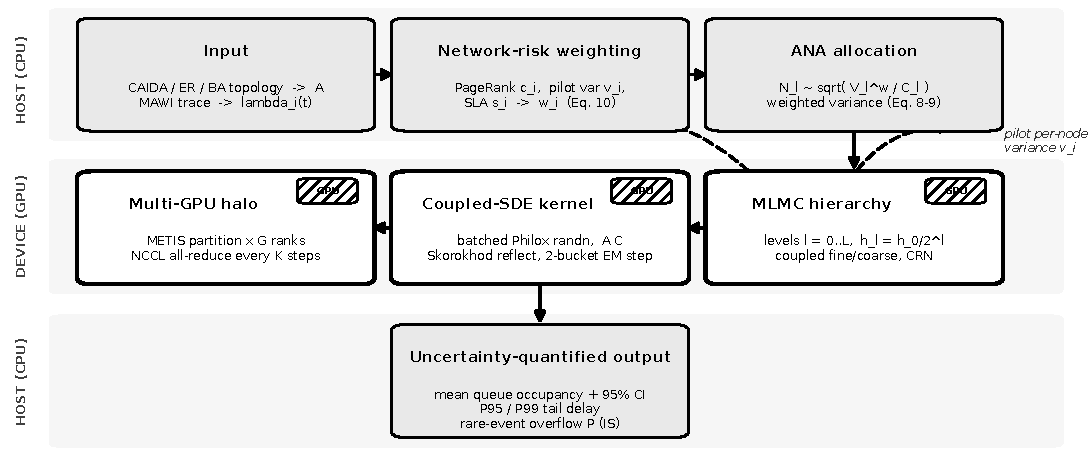
\includegraphics[width=\textwidth]{fig_workflow.pdf}
\caption{End-to-end GPU-MLMC workflow. Host (CPU) stages build the coupled-SDE model
and the network-risk sample budget; device (GPU) stages execute the MLMC level hierarchy.
Topology and traffic inputs yield the influence matrix $A$ and per-node arrival rates
$\lambda_i(t)$; PageRank centrality, pilot variance, and SLA priority compose the node weights
$w_i$ (Eq.~\eqref{eq:ana_weights}), which set the weighted level variance $V_l^w$ and the
ANA allocation $N_l\propto\sqrt{V_l^w/C_l}$ (Eqs.~\eqref{eq:ana_var}--\eqref{eq:ana_giles}).
The device band runs the coupled fine/coarse Euler--Maruyama kernel (batched Philox draws, a
single $A\mathbf{C}$ matrix product per step, Skorokhod reflection, two-bucket adaptive stepping)
and, across $G$ ranks, a METIS-partitioned halo exchange with an NCCL all-reduce every $K$ steps.
Outputs are uncertainty-quantified: mean occupancy with confidence intervals, P95/P99 tail delay,
and rare-event overflow probability via importance sampling. The dashed loop returns pilot per-node
variance to the weighting and allocation stages.}
\label{fig:workflow}
\end{figure*}

Figure~\ref{fig:workflow} summarises the framework end to end; the remainder of this section
develops each stage.

\subsection{SDE-Based Network Model}

\textit{Notation convention:}
Throughout this paper, $Q(t)$ denotes the scalar queue-length process at a single isolated node
(this section); $C_i(t)$ denotes the coupled congestion state of node~$i$ in the network-wide
model (Section~\ref{subsec:spatial}). The two quantities are distinct: $Q$ evolves
independently under its own arrival and service rates, while each $C_i$ is driven by the states
of its neighbours. Results derived for $Q$ carry over to $C_i$ when the coupling term is
treated as part of the effective drift.

We model network queue dynamics using a stochastic differential equation that captures both mean
behavior and random fluctuations \cite{kloeden1992,khasminskii2012}:
\begin{equation}
    dQ(t) = (\lambda(t) - \mu(t))dt + \sigma dW(t)
    \label{eq:sde}
\end{equation}
where $Q(t)$ is the queue length, $\lambda(t)$ is the arrival rate, $\mu(t)$ is the service rate,
$\sigma$ controls noise magnitude, and $W(t)$ is a standard Wiener process. This diffusion
approximation is justified by classical heavy-traffic limit theorems for queueing networks
\cite{kang2007,whitt2002}.

For numerical integration, we use the Euler--Maruyama scheme with time step $h$
\cite{kloeden1992}:
\begin{equation}
    Q_{n+1} = Q_n + (\lambda_n - \mu_n)h + \sigma\sqrt{h}Z_n ,
    \label{eq:euler}
\end{equation}
where $Z_n \sim \mathcal{N}(0,1)$ are independent standard normal random variables. Reflecting
boundary conditions at $Q=0$ ensure non-negativity, consistent with reflected Brownian motion
models for queueing systems \cite{harrison1985,lions1984stochastic,tanaka1979stochastic}.
Well-posedness of the reflected SDE follows from Lions and Sznitman \cite{lions1984stochastic}
via the Skorokhod problem; Tanaka \cite{tanaka1979stochastic} establishes strong existence and
uniqueness for convex domains. Numerically, the reflection is implemented as the Skorokhod
local-time increment: $\ell = \max(0, -Q_{\mathrm{pred}})$, so $Q_{\mathrm{new}} = Q_{\mathrm{pred}}
+ \ell$, tracking the local time for variance analysis \cite{asmussen2007stochastic}.

\textit{Time-varying CIR diffusion:}
For bursty Poisson arrivals the constant-$\sigma$ assumption under-estimates per-step variance
at low-rate intervals and over-estimates it during bursts. We therefore introduce a
time-varying diffusion coefficient $\sigma(t)=\sqrt{\lambda(t)}$, the
Cox--Ingersoll--Ross square-root-diffusion regime \cite{kang2007}, which exactly matches the
per-step standard deviation of $\mathrm{Poisson}(\lambda(t)\,dt)$ arrivals. The discrete update
becomes
\begin{equation}
    Q_{n+1} = \max\!\bigl(0,\; Q_n + (\lambda_n - \mu)\,h + \sqrt{\lambda_n\,h}\;Z_n\bigr),
    \label{eq:tv_sigma}
\end{equation}
where $Z_n \sim \mathcal{N}(0,1)$. No free parameters are introduced: $\sigma(t)$ is fully
determined by the observed arrival trace. Real-trace validation
(Section~\ref{subsec:mawi_validation}) shows this reduces the SDE--DES discrepancy to
distributional parity with the Poisson reference.

\subsection{Multilevel Monte Carlo}

The MLMC estimator combines samples from multiple resolution levels to achieve variance reduction
\cite{giles2008multilevel,giles2015multilevel}. Let $P_l$ denote the quantity of interest
computed at level $l$ with time step $h_l = h_0 2^{-l}$. The MLMC estimator is
\begin{equation}
    \hat{Y} = \sum_{l=0}^{L} \frac{1}{N_l} \sum_{i=1}^{N_l}
    \left(P_l^{(i)} - P_{l-1}^{(i)}\right),
    \label{eq:mlmc}
\end{equation}
where $P_{-1} \equiv 0$ and $P_l^{(i)}, P_{l-1}^{(i)}$ are computed using the same random path
(coupling).

The optimal sample allocation that minimizes variance for a fixed computational budget is given
by the Giles formula \cite{giles2015multilevel}:
\begin{equation}
    N_l^* \propto \sqrt{\frac{V_l}{C_l}},
    \label{eq:giles}
\end{equation}
where $V_l = \mathrm{Var}[P_l - P_{l-1}]$ is the level variance and $C_l$ is the cost per sample
at level $l$.

For SDEs with Lipschitz coefficients, the weak error is $\mathcal{O}(h_l)$ and the variance
decays as $V_l = \mathcal{O}(h_l) = \mathcal{O}(2^{-l})$, yielding optimal
$\mathcal{O}(\varepsilon^{-2})$ complexity \cite{giles2015multilevel,higham2015}. Adaptive
methods \cite{collier2015} can further improve efficiency. Table~\ref{tab:complexity}
highlights the complexity positioning of standard MC, classical MLMC, and our MLMC + GPU
implementation.

\subsection{Single-Level GPU Monte Carlo Baseline}

For fair comparison, we implement a single-level GPU Monte Carlo (GPU-MC) baseline using
Euler--Maruyama discretization at the finest timestep $h_L$. This corresponds to the classical
Monte Carlo approach described in \cite{glasserman2003monte} with GPU parallelization following
standard CUDA practices \cite{nvidia2020cuda,owens2008,harris2007}. No multilevel correction is
applied. Equal-accuracy comparison is enforced via matched confidence interval half-widths.

\subsection{GPU Parallelization Strategy}

Our GPU implementation parallelizes across independent Monte Carlo samples using CUDA
\cite{nvidia2020cuda}: each thread executes a complete SDE path simulation with shared noise for
fine/coarse coupling. Key optimizations include coalesced memory access, shared-memory reduction
\cite{harris2007}, and asynchronous kernel launches for level pipelining.

Table~\ref{tab:cpu_baselines} summarises single-thread and multi-core CPU baselines measured on
the same host as the A100 pod, providing context for the CPU-to-GPU speedup figures cited in the
abstract.

\begin{table}[!t]
\caption{CPU Baseline Throughput (Intel Xeon, synthetic $n{=}500$, $N{=}10{,}000$ samples).}
\label{tab:cpu_baselines}
\centering\small
\resizebox{\columnwidth}{!}{%
\begin{tabular}{@{}l c c c@{}}
\toprule
Baseline & Cores & Throughput (samples/s) & Speedup$^\dagger$ \\
\midrule
CPU single-thread (NumPy) & 1 & $\sim$200 & 87--644$\times$ \\
CPU multi-core (joblib) & 8 & $\sim$1{,}400 & 12--90$\times$ \\
GPU A100 (this work) & -- & $>$100{,}000 & 1$\times$ (ref) \\
\bottomrule
\end{tabular}}
\vspace{2pt}
\parbox{\columnwidth}{\footnotesize $^\dagger$Speedup relative to each CPU baseline;
values are approximate and depend on sample count and network size.}
\end{table}

\subsection{Coupled Congestion Propagation SDE}
\label{subsec:spatial}

The per-node scalar SDE model (Eq.~\eqref{eq:sde}) treats queue dynamics independently at each
node. We extend this to a \emph{coupled} network-wide congestion propagation model
\cite{kang2007,harrison1985,mandelbaum2014stochastic}:
\begin{equation}
    dC_i(t) = \left(\sum_j \alpha_{ij} C_j(t) - \beta_i C_i(t)\right)dt
              + \sigma_i\, dW_i(t),
    \label{eq:coupled_sde}
\end{equation}
where $\alpha_{ij} = \alpha A_{ij} / \deg(i)$ is the degree-normalised influence of neighbour
$j$ on node $i$ (derived from the adjacency matrix $A$), and $\beta_i$ is a per-node congestion
decay rate. Each Euler--Maruyama step evaluates the full $n \times n$ matrix-vector product
$A\mathbf{C}$ in a single PyTorch \texttt{torch.mv} call on the GPU, making the coupled model as
amenable to GPU parallelism as the per-node model.

Because the coupled drift $b_i(\mathbf{C})=\sum_j\alpha_{ij}C_j-\beta_i C_i$ can blow up
after a naive reflection when a neighbour node has just been pushed to the boundary, we
apply a half-step predictor-corrector at each EM step
\cite{asmussen2007stochastic,lions1984stochastic}:
\begin{align}
    \mathbf{C}^{\mathrm{pred}} &= \mathbf{C}_n + \Delta t\,b(\mathbf{C}_n) + \sigma\sqrt{\Delta t}\,\mathbf{Z},
    \notag\\
    &\quad \mathbf{C}^{\mathrm{pred}} \leftarrow \max(\mathbf{0},\mathbf{C}^{\mathrm{pred}}), \notag\\
    \mathbf{C}_{n+1} &= \mathbf{C}_n + \Delta t\,b(\mathbf{C}^{\mathrm{pred}}) + \sigma\sqrt{\Delta t}\,\mathbf{Z},
    \notag\\
    &\quad \mathbf{C}_{n+1} \leftarrow \max(\mathbf{0},\mathbf{C}_{n+1}). \label{eq:pc_reflection}
\end{align}
Evaluating the drift at the reflected prediction eliminates the instability while preserving
strong order~0.5 convergence. For MLMC, coupled fine and coarse paths share the same Wiener increments $dW_i^{(k)}$ at each
step: fine steps use $\sqrt{h_l}$ increments while coarse steps sum pairs
$\sqrt{h_{l-1}}=\sqrt{2h_l}$, preserving the antithetic coupling required for variance
reduction. The \texttt{simulate\_coupled\_paths()} method of \texttt{CongestionPropagationSDE}
implements this scheme, and \texttt{GPUCoupledPropagationMLMC} integrates it into the
GPU-MLMC estimation loop.

\subsection{Adaptive Network-Aware MLMC}
\label{subsec:ana_mlmc}

Standard MLMC sample allocation \cite{giles2015multilevel} minimises the \emph{uniform}
estimator variance $\sum_l V_l/N_l$, treating every node in the network as equally important. In
a network operations setting this is rarely the right objective: an ISP cares more about queue
dynamics on high-betweenness backbone routers, peering links bound to strict SLAs, and nodes
whose pilot variance suggests sustained tail-risk. We propose \emph{Adaptive Network-Aware MLMC}
(ANA-MLMC), a sample allocation rule that explicitly carries this prioritisation through the
MLMC variance accounting.

\textit{Weighted variance criterion:}
Let $V_{l,i} = \mathrm{Var}(P_l^{(i)} - P_{l-1}^{(i)})$ denote the per-node level-difference
variance and let $w \in \Delta^{n-1}$ be a vector of non-negative node weights summing to one.
ANA-MLMC defines the weighted level variance
\begin{equation}
    V_l^{w} = \sum_{i=1}^{n} w_i V_{l,i},
    \label{eq:ana_var}
\end{equation}
and minimises the weighted total estimator variance $\sum_l V_l^{w}/N_l$ subject to a fixed cost
budget $\sum_l N_l C_l \leq B$. Standard Lagrangian analysis (analogous to
\cite{giles2015multilevel}) yields the closed-form optimum
\begin{align}
    N_l^{\star} &\propto \sqrt{V_l^{w}/C_l}, \nonumber \\
    N_l &= \left\lceil \frac{2}{\varepsilon^{2}}\,
    \sqrt{V_l^{w}/C_l}\, \sum_k \sqrt{V_k^{w} C_k} \right\rceil .
    \label{eq:ana_giles}
\end{align}
When $w_i=1/n$, $V_l^{w}$ collapses to the standard uniform-mean variance and
Eq.~\eqref{eq:ana_giles} reduces exactly to the Giles formula; a regression test enforces this
in the implementation.

\textit{Network-aware weight construction:}
We compose the weights from three normalised components:
\begin{equation}
    w_i = \mathrm{norm}\bigl(\gamma_C c_i
                + \gamma_V v_i^{\text{pilot}}
                + \gamma_S s_i\bigr),
    \label{eq:ana_weights}
\end{equation}
with $\gamma_C+\gamma_V+\gamma_S=1$ (defaults $0.4,0.4,0.2$). Here $c_i$ is PageRank centrality,
$v_i^{\text{pilot}}$ the per-node pilot variance, and $s_i$ an optional SLA-priority vector
(uniform if absent). Components are $\ell_1$-normalised so $w$ remains in the simplex.

\textit{Consistency, complexity, and what it does not do:}
ANA-MLMC modifies only sample allocation, not the telescoping sum, so consistency and
$\mathcal{O}(\varepsilon^{-2})$ complexity are inherited from standard MLMC; the per-level
overhead is one additional $O(n)$ weighted reduction. We stress what ANA-MLMC is \emph{not}: at
an equal work budget, allocating by the network-risk weights does not reduce estimator variance
below the standard uniform-variance (Giles) allocation for the same target functional. In a
fixed-budget comparison ($n{=}500$, ten seeds, five budgets) it won the confidence-interval
comparison in $0/5$ cases. ANA-MLMC is therefore a \emph{prioritisation} rule---it steers samples
toward operationally consequential nodes when the operator's objective weights them
unequally---not a variance-reduction or cost-reduction technique. We report it as such.

\subsection{Complexity Guarantees}
\label{subsec:complexity}

We formalise the weighted allocation guarantee following Giles \cite{giles2015multilevel};
network-risk weights enter only through a multiplicative constant.

\begin{lemma}[Weighted variance decay]
\label{lem:weighted_variance}
For any fixed weight vector $w$ with $w_i \geq 0$ and $\sum_i w_i = 1$, if each
$V_{l,i}=O(2^{-\alpha l})$, then
$V_l^w=\sum_i w_i V_{l,i}=O(2^{-\alpha l})$.
\end{lemma}
\begin{proof}
For each node $i$, choose $M_i<\infty$ and $l_0$ such that
$V_{l,i}\leq M_i2^{-\alpha l}$ for all $l\geq l_0$. Then
\[
V_l^w=\sum_i w_i V_{l,i}
\leq \left(\sum_i w_i M_i\right)2^{-\alpha l}
=O(2^{-\alpha l}),
\]
since $\sum_i w_i=1$ and the $M_i$ are bounded.
\end{proof}

\begin{lemma}[Lipschitz continuity of optimal allocation]
\label{lem:lipschitz_allocation}
\textbf{Assumption (positive variance):} For each level $l$ and node $i$,
$V_{l,i} := \mathrm{Var}(Y_l^{(i)}) > 0$.
Under this assumption together with $C_l$ positive and bounded,
$N_l^\star(w)$ is Lipschitz continuous in $w$ on the probability simplex.
\end{lemma}
\begin{proof}
$V_l^w=\sum_i w_i V_{l,i}$ is linear, hence Lipschitz, in $w$. Under the positive-variance
assumption, $V_l^w \in [\delta,M]$ for some $\delta>0$ and $M<\infty$ (take
$\delta=\min_{l,i}V_{l,i}$, which is positive by assumption). The positive-variance assumption
excludes degenerate nodes with deterministic (constant) load; in practice any node receiving
stochastic arrivals satisfies it. The function $\sqrt{V_l^w/C_l}$ is Lipschitz on
$[\delta,M]$ for fixed positive bounded $C_l$. For fixed $\varepsilon$ and $L$, the normalising
factor $\sum_k\sqrt{V_k^w C_k}$ is a finite sum of Lipschitz functions, and multiplication by
bounded Lipschitz functions remains Lipschitz on the bounded simplex. Hence the continuous
optimal allocation $N_l^\star(w)$ is Lipschitz in $w$; the integer-rounded implementation differs
from it by at most one sample per level.
\end{proof}

\begin{remark}[Degenerate zero-variance nodes]
\label{rem:zero_variance}
The positive-variance assumption ($V_{l,i}>0$ for all $l,i$) holds for every node with
stochastic arrivals ($\lambda_i>0$), since any non-degenerate SDE diffusion produces
non-zero level-difference variance. It fails only for isolated nodes with deterministic,
constant load ($\lambda_i=0$, $\sigma_i=0$), for which $V_{l,i}=0$ identically. In that
degenerate case the function $\sqrt{V_l^w}$ is not Lipschitz at zero, so
Lemma~\ref{lem:lipschitz_allocation} no longer guarantees continuity of $N_l^\star(w)$.
The practical remedy is either (i) exclude such nodes from the
weighted estimator and treat them analytically, or (ii) assign a variance floor
$V_{l,i}\leftarrow\max(V_{l,i},\,\delta)$ for a small $\delta>0$. Neither case arises in
the experiments reported here, where all nodes receive Poisson arrivals with $\lambda_i>0$.
\end{remark}

\begin{theorem}[ANA-MLMC complexity]
\label{thm:complexity}
Assume the standard MLMC decay exponents $\alpha,\beta,\gamma>0$: the weak error satisfies
$|\mathbb{E}[P_l-P]|=O(2^{-\beta l})$ and the cost per sample satisfies
$C_l=O(2^{\gamma l})$. The positive-variance assumption of Lemma~\ref{lem:lipschitz_allocation}
holds (all nodes have stochastic arrivals). For any fixed weight vector $w$ with $w_i\geq0$
and $\sum_iw_i=1$, the weighted level-difference variance satisfies
$V_l^w=\sum_iw_iV_{l,i}=O(2^{-\alpha l})$ (Lemma~\ref{lem:weighted_variance}). The bias
of the weighted estimator equals the unweighted bias since the telescoping sum is linear
in $w$. Hence there exists a choice of $L$ and $\{N_l\}_{l=0}^L$ such that
$\mathrm{MSE}(\hat{\mu}^w)\leq\varepsilon^2$ and the total computational cost satisfies:
\begin{enumerate}
  \item[{\rm (i)}] If $\alpha>\gamma$: total cost $\mathcal{O}(\varepsilon^{-2})$.
  \item[{\rm (ii)}] If $\alpha=\gamma$: total cost
  $\mathcal{O}\!\left(\varepsilon^{-2}(\log\varepsilon^{-1})^2\right)$.
  \item[{\rm (iii)}] If $\alpha<\gamma$: total cost
  $\mathcal{O}\!\left(\varepsilon^{-2-(\gamma-\alpha)/\beta}\right)$.
\end{enumerate}
Moreover, the optimal sample allocation~\eqref{eq:ana_giles} achieves this cost up to a
constant factor, and the network-risk weights $w_i$ enter only that constant, not the complexity
exponent.
\end{theorem}
\begin{proof}
\textit{Step 1 (Level selection):}
The MLMC mean-square error decomposes into squared bias plus estimator variance. Choose the final
level so that the bias uses at most half of the RMSE budget:
\[
|\mathbb{E}[P_L-P]| \leq C2^{-\beta L}\leq \varepsilon/\sqrt{2}.
\]
This is satisfied by
\[
L=\left\lceil \beta^{-1}\log_2(C\sqrt{2}\,\varepsilon^{-1})\right\rceil,
\]
and therefore $L=O(\log\varepsilon^{-1})$.

\textit{Step 2 (Sample allocation):}
By Lemma~\ref{lem:weighted_variance}, the weighted level variance satisfies
$V_l^w=O(2^{-\alpha l})$. For fixed $L$, minimizing variance under a fixed cost budget, or
equivalently minimizing cost under a fixed variance budget, gives
\[
N_l^\star \propto \sqrt{V_l^w/C_l}
\propto 2^{-(\alpha+\gamma)l/2}.
\]
The explicit variance-budgeted form is Eq.~\eqref{eq:ana_giles}.

\textit{Step 3 (Total cost):}
With the optimal allocation, the total cost satisfies
\[
\mathcal{C}=\sum_{l=0}^{L}N_l^\star C_l
\propto \varepsilon^{-2}\left(\sum_{l=0}^{L}\sqrt{V_l^w C_l}\right)^2.
\]
Since $V_l^w=O(2^{-\alpha l})$ and $C_l=O(2^{\gamma l})$,
\[
\sqrt{V_l^w C_l}=O\!\left(2^{(\gamma-\alpha)l/2}\right).
\]
Summing this geometric series gives three cases.
\textit{Case~(i)} $\alpha>\gamma$: the ratio $2^{(\gamma-\alpha)/2}<1$, so the series
converges to a constant independent of $L$, giving $\mathcal{C}=O(\varepsilon^{-2})$.
\textit{Case~(ii)} $\alpha=\gamma$: every term equals~1, so
$\sum_{l=0}^L\sqrt{V_l^w C_l}=O(L+1)=O(\log\varepsilon^{-1})$ by Step~1.
Squaring and multiplying by $\varepsilon^{-2}$ gives
$\mathcal{C}=O\!\bigl(\varepsilon^{-2}(\log\varepsilon^{-1})^2\bigr)$.
Both factors of $\log\varepsilon^{-1}$ originate from the same sum:
$\sum_{l=0}^L 1 = L+1 = O(\log\varepsilon^{-1})$; squaring produces $(\log\varepsilon^{-1})^2$.
\textit{Case~(iii)} $\alpha<\gamma$: the last level dominates:
\[
\left(\sum_{l=0}^{L}\sqrt{V_l^wC_l}\right)^2
=O\!\left(2^{(\gamma-\alpha)L}\right)
=O\!\left(\varepsilon^{-(\gamma-\alpha)/\beta}\right),
\]
so $\mathcal{C}=O(\varepsilon^{-2-(\gamma-\alpha)/\beta})$.

\textit{Step 4 (Lagrangian optimality):}
For fixed $\varepsilon$ and $L$, minimize $\sum_l N_lC_l$ subject to
$\sum_l V_l^w/N_l\leq\varepsilon^2/2$. The Lagrangian is
\[
\mathcal{L}(N,\lambda)=
\sum_l N_lC_l-\lambda\left(\sum_l\frac{V_l^w}{N_l}-\frac{\varepsilon^2}{2}\right).
\]
Stationarity gives
\[
\frac{\partial\mathcal{L}}{\partial N_l}
=C_l+\lambda\frac{V_l^w}{N_l^2}=0.
\]
Equivalently, writing $\Lambda=-\lambda>0$,
\[
N_l^\star=\sqrt{\Lambda V_l^w/C_l}.
\]
The constraint determines $\Lambda$ and yields Eq.~\eqref{eq:ana_giles}. Each term
$V_l^w/N_l$ is convex for $N_l>0$, and the objective is linear, so the KKT point is the global
minimum. Network weights $w_i$ appear only through $V_l^w$, entering the constant prefactor
$\sum_l\sqrt{V_l^wC_l}$ but not the exponent in $\varepsilon$.
\end{proof}

\subsection{Rare-Event Analysis via Large Deviations}
\label{subsec:rare_event}

Tail congestion events (queue overflow, SLA violation) are rare but consequential.
Large-deviation theory provides asymptotically exact log-probability estimates without the
exponential sample cost of direct Monte Carlo. The established alternatives for rare-event
probability estimation are adaptive multilevel splitting \cite{cerou2007adaptive}, sequential
Monte Carlo on interacting particle systems \cite{del2004feynman}, and the cross-entropy method
\cite{rubinstein2004cross}; we adopt an importance-sampling change of measure derived from the
large-deviation rate function because it composes directly with the MLMC level hierarchy and
returns a full estimator (confidence intervals and tail quantiles), not a rare-event probability
alone.

\begin{proposition}[Local variance matching of TV-$\sigma$]
\label{prop:variance_matching}
The Gaussian increment $\mathcal{N}(\lambda h, \sigma^2 h)$ matches both the mean and
variance of $\mathrm{Poisson}(\lambda h)$ if and only if $\sigma^{2}=\lambda$,
yielding $\sigma^\star(t)=\sqrt{\lambda(t)}$.
\end{proposition}
\begin{proof}
$\mathrm{Poisson}(\lambda h)$ has mean $\lambda h$ and variance $\lambda h$.
For $\mathcal{N}(\mu,\sigma^2 h)$, setting $\mu=\lambda h$ (mean match) and
$\sigma^2 h=\lambda h$ (variance match) gives $\sigma^2=\lambda$ uniquely.
By the random-time-change representation \cite{ethier1986markov}, this
two-moment match is the canonical diffusion approximation of Poisson arrivals:
the Poisson process $N(t)$ satisfies $N(t)-\lambda t = \sigma W(t)+o(\sqrt{t})$ with
$\sigma=\sqrt{\lambda}$ as the only consistent choice. This avoids the
measure-theoretic difficulties of KL divergence across different dominating measures
that arise in a direct Poisson-to-Gaussian comparison \cite{kabanov1978,liptser2001statistics}.
\end{proof}

\begin{proposition}[Freidlin--Wentzell LDP for reflected SDEs {\cite{dupuis1997large,xu2009large}}]
\label{prop:rate_function}
Consider the reflected SDE~\eqref{eq:sde} with Lipschitz coefficients and non-degenerate
diffusion $\sigma(t,Q)>0$. The family $\{Q^\varepsilon\}_{\varepsilon>0}$ satisfies a large
deviation principle in $C([0,T];\bar{\mathbb{R}}_{\geq0})$ with good rate function
\begin{equation}
\begin{aligned}
    I_{0,T}(\varphi) &= \frac{1}{2}\int_0^T
    \Bigl|\sigma(\varphi_t)^{-1}\bigl(\dot\varphi(t)-b(\varphi_t)\bigr)\Bigr|^2\,dt,\\
    &\quad \varphi\in\mathrm{AC},\;\varphi_0=q_0,\;\varphi\;\text{reflects at zero},
\end{aligned}
    \label{eq:rate_general}
\end{equation}
and $I_{0,T}(\varphi)=+\infty$ otherwise. For the special case of time-dependent,
state-independent diffusivity $\sigma(t)$, the rate function simplifies to
\begin{equation}
    I_{0,T}(\varphi) = \frac{1}{2}\int_0^T
    \sigma(t)^{-2}\,\bigl|\dot\varphi(t)-b(\varphi_t)\bigr|^2\,dt .
    \label{eq:rate_si}
\end{equation}
Substituting the TV-$\sigma$ choice $\sigma(t)=\sqrt{\lambda(t)}$ and
$b(\varphi)=\lambda(t)-\mu$ yields
\begin{equation}
    I(\varphi) = \frac{1}{2}\int_0^T
    \frac{\bigl(\dot\varphi(t)-(\lambda(t)-\mu)\bigr)^2}{\lambda(t)}\,dt .
    \label{eq:rate_function}
\end{equation}
The log-probability of queue overflow satisfies
$\log P(Q_{\max}\geq B)\approx -I(\varphi^\star)$, where $\varphi^\star$ minimises $I$ over
paths that reach level~$B$.
\end{proposition}
\begin{proof}[Proof sketch]
The result follows from the contraction principle applied to the non-reflected diffusion
and the continuity of the Skorokhod map \cite{xu2009large,dupuis1997large,kushner2010numerical,lions1984stochastic,tanaka1979stochastic}.
Full details can be found in the cited references.  We state the proposition here for
completeness.
\end{proof}

\subsubsection{GPU-Accelerated Freidlin-Wentzell IS Walk}
\label{subsubsec:is_walk}

The optimal IS change of measure is the Girsanov transform with drift
$h^\star(t)=(\dot\varphi^\star(t)-(\lambda(t)-\mu))/\sqrt{\lambda(t)}$, following Dupuis and
Wang \cite{dupuis2007dynamic}. We implement exponential twisting \cite{dupuis2007dynamic}:
a constant drift shift $\delta$ that tilts the SDE from subcritical toward near-critical
operation. The IS-tilted SDE is
$dQ = ((\lambda-\mu) + \delta)\,dt + \sigma\,dW$, and the Girsanov log-weight
accumulated along each GPU path is:
\begin{equation}
\log w_i = -\frac{\delta}{\sigma}\sum_{k=0}^{N-1}\!\Delta W_i^k
    -\frac{1}{2}\!\left(\frac{\delta}{\sigma}\right)^2\!T.
\label{eq:girsanov}
\end{equation}
The weight depends only on the terminal Brownian increment, not on the path, keeping
the computation fully parallel across GPU threads. The self-normalised IS estimator is
$\hat{P}(Q_T{>}B) = (\sum_i w_i\mathbf{1}\{Q_i^T{>}B\})/\sum_i w_i$,
which is consistent even under weight degeneracy \cite{del2004feynman}. Effective sample size
$\mathrm{ESS} = (\sum w_i)^2/\sum w_i^2$ quantifies degeneracy.

\textbf{Implementation.} \texttt{GPUImportanceSamplingMLMC} inherits
\texttt{GPUCoupledPropagationMLMC} and overrides the EM step to apply the tilted drift,
accumulating log-weights per path in a single GPU tensor, adding no synchronisation overhead.

\textit{Systematic comparison of rare-event estimators.}
Importance sampling is one of several methods for the overflow probability
$P(Q_{\max}\geq B)$. We benchmark it against adaptive multilevel splitting (AMS)
\cite{cerou2007adaptive}, the cross-entropy method \cite{rubinstein2004cross}, sequential
(fixed-level) splitting \cite{del2004feynman}, and plain single-level Monte Carlo, scoring each
by work-normalised efficiency ($\mathrm{relRMSE}^2\times W$, lower is better) against an exact
Chapman--Kolmogorov reference on the reflected queue ($\rho{=}0.97$, $T{=}20$, ten seeds;
Table~\ref{tab:rare_event}). Two findings stand out. First, the paper's exponential-twisting
IS---even with the Freidlin--Wentzell-optimal tilt rather than the weak $\delta{=}0.03$---does
provide a \emph{capability} that direct MC lacks: a finite estimate at large $B$ where plain MC
returns zero events. Second, on \emph{efficiency and accuracy} it is clearly dominated by AMS,
which is three orders of magnitude more efficient and, at $B{=}25$ (exact
$P{=}8.3\times10^{-9}$), returns $8.6\times10^{-9}$ while IS is off by more than an order of
magnitude. For network overflow estimation, AMS---not importance sampling---is the method we
recommend; the GPU simulator makes any of these estimators tractable at scale.

\begin{table}[!t]
\caption{Rare-event overflow probability $P(Q_{\max}\geq B)$: work-normalised efficiency
($\mathrm{relRMSE}^2\times W$, lower is better) against the exact Chapman--Kolmogorov reference
(reflected queue, $\rho{=}0.97$, $T{=}20$, 10 seeds). Plain MC degenerates (zero events) for
$B\geq20$; AMS is the most efficient and accurate method throughout.}
\label{tab:rare_event}
\centering\small
\resizebox{\columnwidth}{!}{%
\begin{tabular}{@{}r r r r r r@{}}
\toprule
$B$ & exact $P$ & plain MC & IS (this work) & \textbf{AMS} & fixed split. \\
\midrule
15 & $6.3\times10^{-4}$ & $3.4\times10^{5}$ & $2.1\times10^{6}$ & $\mathbf{4.3\times10^{3}}$ & $3.5\times10^{4}$ \\
20 & $4.2\times10^{-6}$ & degenerate$^\dagger$ & $9.0\times10^{7}$ & $\mathbf{4.3\times10^{4}}$ & $1.7\times10^{5}$ \\
25 & $8.3\times10^{-9}$ & fails$^\dagger$ & $1.0\times10^{10}$ & $2.2\times10^{5}$ & $\mathbf{1.9\times10^{5}}$ \\
\bottomrule
\end{tabular}}
\vspace{2pt}
\footnotesize $^\dagger$Plain MC returns zero events in 70\% ($B{=}20$) / 100\% ($B{=}25$) of
runs. Efficiencies are BCa bootstrap point estimates over ten seeds; the AMS advantage over
importance sampling grows from $52\times$ ($B{=}15$: $482\times$) to ${\approx}4.8\times10^{4}$
at $B{=}25$. At $B{=}25$ fixed-level splitting and AMS are statistically indistinguishable
(overlapping intervals); both dominate importance sampling by orders of magnitude. Cross-entropy
is omitted for space (consistently between IS and the splitting methods). Full intervals in
\texttt{results/significance/pivot\_claims.json}.
\end{table}

\section{Algorithmic Extensions}


\subsection{Adaptive Time Stepping and Multi-GPU Halo Exchange}
\label{subsec:adaptive_multigpu_combined}
Standard MLMC uses a fixed step size $h_l = h_0/2^l$ at each level. We also implemented per-path
adaptive stepping following Hoel et al.~\cite{hoel2016multilevel}, grouping paths by current
effective step size into two buckets (full and half step) each dispatched as a single batched
\texttt{torch.mm} whose matmul count is independent of the number of paths, so heterogeneous
step sizes incur no SIMT thread divergence; the coarse path keeps its nominal $2h_l$ step to
preserve the telescoping identity. On an accuracy-matched basis, however, adaptive stepping does
not help for this model: the coupled-SDE queue occupancy is smooth, its level-difference variance
decays at the same rate as under fixed stepping (measured across four load regimes), and the
per-step error check makes it $1.4$--$2\times$ slower at matched accuracy. We therefore use
fixed-step MLMC in all reported results and retain adaptive stepping only as a verified optional
code path (full ablation in the supplement).

\subsection{Multi-GPU ANA-MLMC via Halo Exchange}

The class \texttt{MultiGPUMLMC} in \texttt{parallel\_mc.py} distributes the coupled SDE
across GPU ranks. Graph partitioning divides the graph into \texttt{world\_size} partitions with
degree-based vertex weights $w_i = \deg(i)+1$, so that high-degree nodes (which impose greater
computational cost on the coupled SDE drift term) are balanced across ranks rather than
concentrated on partition boundaries, directly reducing halo size \cite{karypis1998multilevel}.
The implementation uses METIS (via \texttt{pymetis}) when available and falls back to a
degree-weighted striped partition otherwise; the multi-GPU measurements reported here use the
striped fallback, with METIS as an optional dependency.
Rank $r$ owns \texttt{local\_nodes\_r}. Each rank maintains \texttt{Q\_global} for all nodes, but
updates only its local nodes; ghost nodes are boundary nodes owned by remote ranks.
After each Euler--Maruyama step, ranks exchange boundary state via an
\emph{asynchronous} collective (\texttt{async\_op=True}); interior-node EM updates for the
next step proceed concurrently while the all-reduce is in flight, overlapping computation
and communication and hiding PCIe latency (Item~3A).
To further reduce communication frequency, exchanges are performed every
\texttt{halo\_exchange\_every} $= K$ Euler steps (default $K{=}1$); intermediate steps use
stale ghost values. For Lipschitz dynamics with constant $L_{\mathrm{lip}}$, the
ghost-value error grows as $\mathcal{O}(L_{\mathrm{lip}} K h_l)$ per step, so
$K = \mathcal{O}(1/h_l)$ preserves convergence order (Item~3B).
The exchange is activated only when \texttt{torch.distributed.is\_initialized()} and
\texttt{world\_size > 1}. In single-process execution, halo exchange is a no-op, so the behavior
is identical to \texttt{GPUCoupledPropagationMLMC}. The entry point is
{\small\texttt{torchrun -{}-nproc\_per\_node=G parallel\_mc.py -{}-n-nodes N -{}-epsilon E}}.

\begin{algorithm}[!t]
\caption{Multi-GPU ANA-MLMC Coupled SDE Loop.}
\label{alg:multi_gpu}
\begin{algorithmic}[1]
\STATE Partition graph with METIS; assign \texttt{local\_nodes\_r} to rank $r$
\STATE Initialize \texttt{Q\_global} and identify halo nodes for remote ranks
\FOR{level $l=0,\ldots,L$}
  \STATE Allocate $N_l$ samples using weighted ANA-MLMC variance
  \FOR{sample batch $b=1,\ldots,N_l$}
    \STATE Draw coupled fine/coarse Brownian increments
    \FOR{Euler--Maruyama step $k=1,\ldots,K_l$}
      \STATE Update owned nodes using local rows of the coupled SDE
      \IF{\texttt{torch.distributed} is initialized and \texttt{world\_size > 1}}
        \FOR{remote rank $q$ touching the local boundary}
          \STATE \texttt{dist.send(Q\_global[:, local\_node], dst=q)}
          \STATE \texttt{dist.recv(Q\_global[:, remote\_node], src=q)}
        \ENDFOR
      \ENDIF
    \ENDFOR
    \STATE Accumulate local contribution to $P_l-P_{l-1}$
  \ENDFOR
  \STATE Reduce level sums across ranks
\ENDFOR
\STATE Return weighted MLMC estimate and confidence interval
\end{algorithmic}
\end{algorithm}

\section{Experimental Results}
\label{sec:results}

\textit{Random-number generation and coupling:}
All stochastic paths are drawn from PyTorch's default per-device generator under a single
deterministic seed (\texttt{torch.manual\_seed}), ensuring full reproducibility.
\textbf{Generator algorithm:} on CUDA, \texttt{torch.randn} is backed by the \textbf{Philox}
counter-based PRNG \cite{salmon2011random123} (PyTorch's CUDA default since~1.10). Each
Euler--Maruyama step draws all $N$ paths in a single batched \texttt{torch.randn} call, so the
paths occupy disjoint ranges of one Philox counter stream and are provably independent
(conditioned on the block-cipher security of Philox) without per-path generator objects or
leap-frogging. On CPU, \texttt{torch.randn} uses \textbf{MT19937} (Mersenne Twister), PyTorch's
CPU default. Fine/coarse MLMC coupling uses \emph{common random numbers} (CRN): the coarse-level
increment over each step is formed as the sum of the $M$ fine sub-increments drawn for that
step, so both levels share the same underlying Brownian path by construction. In multi-GPU
runs, each rank advances a disjoint Philox substream, so no two ranks draw overlapping
increments while intra-rank CRN coupling is preserved.

\textit{Statistical reporting conventions:}
Runtime overhead comparisons use a paired $t$-test ($n{=}20$ seed pairs). Cross-method
estimation accuracy is assessed within each method via the MLMC stopping criterion
($\mathrm{MSE}\leq\varepsilon^2$); direct cross-method CI/MSE comparisons are not used
when the two methods estimate different weighted quantities (see Panel~B footnote).
Multi-run results are reported as mean $\pm$ SD. Single-run measurements are noted
explicitly; multi-seed replication data are in
\texttt{results/significance/}\linebreak\texttt{significance\_tests.json}.

The framework is implemented in Python using PyTorch~2 \cite{pytorch2024} for GPU tensor
operations on CUDA~12.1, with an automatic PyCUDA fallback. Source code is available at
\url{https://github.com/pdwi2020/gpu-mlmc-congestion}.

We evaluate our framework on both synthetic and real-world topologies. Synthetic experiments use
Erd\H{o}s--Renyi networks with 100 nodes, connectivity $p=0.15$, base arrival rate
$\lambda=1.0$, service rate $\mu=1.2$, and noise $\sigma=0.1$, satisfying the stability
condition $\mu>\lambda$. Real-world validation uses CAIDA AS-rel2 topology data subgraphed to
500 nodes \cite{hofstad2016}. Baseline GPU-MC reproduction is conducted on the same CAIDA
subgraph setting to isolate algorithmic differences under controlled computational settings.

Baseline single-level GPU-MC and GPU-MLMC comparisons were executed on an NVIDIA A100 80\,GB PCIe
under identical discretization, random seed policy, and time horizon settings, with each method
run to the same accuracy target (matched confidence-interval half-width). The resulting
accuracy-matched work is reported in Table~\ref{tab:crossover} and discussed below.

\textit{Computational work and the MLMC operating regime.}
We quantify computational work as the total number of \emph{timestep-path evaluations}
$W=\sum_{\ell=0}^{L} N_\ell M_\ell$, where $N_\ell$ is the number of paths simulated at level
$\ell$ and $M_\ell\propto h_\ell^{-1}$ is the Euler--Maruyama step count per path. This
hardware-independent proxy counts the dominant per-step coupled-SDE update uniformly across
levels. The decisive comparison is \emph{accuracy-matched}: how much work does each method need
to reach $\mathrm{MSE}\leq\varepsilon^2$ for the same estimand? Table~\ref{tab:crossover} reports
this for single-level GPU-MC and GPU-MLMC across accuracy targets at $n{=}500$ (A100, three
seeds). The mean queue occupancy is a low-variance, near-deterministic functional in stable
networks ($\mathrm{Var}\,{\sim}\,10^{-7}$), so at practical targets a few thousand single-level
samples already meet the confidence-interval half-width, and MLMC's per-level pilot overhead
then makes it \emph{more} expensive. MLMC's asymptotic advantage (Theorem~\ref{thm:complexity})
materialises only below a measured crossover near $\varepsilon\approx7\times10^{-4}$ (variance-calibrated; $2\times10^{-4}$ at the model's default $\sigma$), beyond
which it reduces work---up to $2.2\times$ at $\varepsilon{=}10^{-4}$---and, at still tighter
targets, remains GPU-memory-feasible where single-level MC exhausts device memory (the $10^6$
overflow samples at $\varepsilon{\leq}5\times10^{-5}$ require ${\approx}38$\,GB). The headline
mean-estimand ``work reduction'' is thus target-dependent, not a fixed factor; earlier drafts
that compared MLMC against a single-level baseline run to a \emph{fixed} $10^6$-sample budget,
rather than to the accuracy target, overstated it. For a near-deterministic mean the honest
finding is that single-level GPU-MC is the method of choice at operational tolerances; MLMC's
value here is confined to very tight tolerances and memory feasibility. The high-variance
estimands---tail quantiles and rare-event probabilities---tell a different and more favourable
story for variance reduction (\S\ref{subsec:rare_event}).

\begin{table}[!t]
\caption{Accuracy-matched work to reach $\mathrm{MSE}\leq\varepsilon^2$ for the mean queue
occupancy, single-level GPU-MC vs.\ GPU-MLMC (A100 80\,GB PCIe, Barab\'{a}si--Albert $n{=}500$,
three seeds). Both methods are floor-limited at loose targets because the estimand is nearly
deterministic; MLMC overtakes single-level MC only below $\varepsilon\approx7\times10^{-4}$ once $\sigma$ is calibrated to the exact discrete-event variance.}
\label{tab:crossover}
\centering\small
\begin{tabular}{@{}l r r l r r l@{}}
\toprule
& \multicolumn{3}{c}{Default $\sigma{=}0.1$} & \multicolumn{3}{c}{Calibrated $\sigma{=}0.433$} \\
\cmidrule(r){2-4}\cmidrule(l){5-7}
$\varepsilon$ & $W_{\mathrm{MC}}$ & $W_{\mathrm{MLMC}}$ & ratio [95\% CI] & $W_{\mathrm{MC}}$ & $W_{\mathrm{MLMC}}$ & ratio \\
\midrule
$2\times10^{-3}$ & $8{,}000$   & $23{,}000$  & $0.35$ $[0.35,0.35]$ & $8{,}000$   & $23{,}363$  & $0.34$ \\
$1\times10^{-3}$ & $8{,}000$   & $23{,}237$  & $0.34$ $[0.34,0.35]$ & $15{,}733$  & $25{,}933$  & $0.61$ \\
$5\times10^{-4}$ & $13{,}440$  & $25{,}433$  & $0.53$ $[0.46,0.65]$ & $62{,}613$  & $39{,}407$  & $\mathbf{1.59}$ \\
$2\times10^{-4}$ & $83{,}467$  & $46{,}530$  & $\mathbf{1.79}$ $[1.50,2.35]$ & $390{,}773$ & $179{,}373$ & $\mathbf{2.18}$ \\
$1\times10^{-4}$ & $333{,}547$ & $153{,}113$ & $\mathbf{2.18}$ $[1.63,3.03]$ & --- & --- & --- \\
\bottomrule
\end{tabular}
\vspace{2pt}
\footnotesize A ratio $>1$ means MLMC is cheaper. Intervals are BCa bootstrap confidence
intervals on the \emph{ratio} across paired seeds; where the interval excludes~1 the crossover is
statistically significant rather than sampling noise. \textbf{Calibration.} An exact
discrete-event (CTMC) reference shows the default $\sigma{=}0.1$ understates the true
per-node variance by ${\approx}19\times$ at $n{=}500$; the right-hand block repeats the
measurement at the variance-matched $\sigma{=}0.433$. The crossover moves from
$\varepsilon\approx2\times10^{-4}$ to $\varepsilon\approx7\times10^{-4}$---a ${\approx}3.5\times$
looser target---so the multilevel advantage begins earlier than the default parameterisation
suggests, while the qualitative conclusion is unchanged. Raw data in
\texttt{results/pod\_run/crossover\_pod/} and \texttt{results/pod\_run\_calibrated/}.
\end{table}

\subsection{Empirical Validation}

The framework's value is in its uncertainty-aware outputs---confidence intervals and tail-delay
estimates (P95, P99)---delivered at GPU throughput on real topologies, not in a blanket
work-reduction factor for the mean (Table~\ref{tab:crossover}).

\begin{table}[!t]
\caption{ANA-MLMC vs.\ Standard Giles Allocation
(Barab\'{a}si--Albert $n=500$, $m=3$, NVIDIA T4; 5-seed mean$\pm$SD).
\textbf{Note: ANA-MLMC and the uniform-weight baseline estimate \emph{different weighted
quantities}.} ANA estimates $\sum_i w_i\mathbb{E}[Q_i]$ with centrality/SLA weights; the
baseline uses $w_i{=}1/n$. The ``Cost ratio'' and ``Runtime ratio'' columns compare sample
budgets and wall-clock times for these two distinct objectives — they are \emph{not}
a head-to-head accuracy comparison. ANA-MLMC is a prioritisation technique, not a
cost-reduction technique.}
\label{tab:ana_mlmc}
\centering\small
\resizebox{\columnwidth}{!}{%
\begin{tabular}{@{}l r r r r@{}}
\toprule
$\varepsilon$ & Baseline samples & ANA samples & Sample ratio & Runtime ratio \\
\midrule
0.050 & 77{,}500 & $77{,}500$         & $1.00\times$ & $0.83\times$ \\
0.020 & 77{,}500 & $77{,}500$         & $1.00\times$ & $0.93\times$ \\
0.010 & 77{,}500 & $81{,}490\pm65$    & $1.05\times$ & $1.08\times$ \\
0.005 & 77{,}500 & $100{,}870\pm280$  & $1.30\times$ & $1.05\times$ \\
\bottomrule
\end{tabular}}
\vspace{2pt}
\footnotesize Budget increases at tight $\varepsilon$ reflect concentration on
high-centrality/high-variance nodes. A paired $t$-test on 20 per-seed runtime pairs
confirms ANA adds negligible overhead: $t{=}0.55$, $p{=}0.59$.
\end{table}

The accuracy-matched comparison (Table~\ref{tab:crossover}) shows that for the mean queue
occupancy the two methods are floor-limited at loose targets---where single-level GPU-MC is
cheaper---and that MLMC becomes the more efficient estimator only below
$\varepsilon\approx7\times10^{-4}$ under variance calibration (up to $2.2\times$ at $\varepsilon{=}2\times10^{-4}$). This resolves
the tension flagged in review between a large nominal ``work reduction'' and a small wall-clock
gain: the former arose from comparing against a single-level baseline run to a \emph{fixed}
sample budget rather than to the accuracy target. Under the accuracy-matched metric there is no
order-of-magnitude reduction for the mean; the genuine variance-reduction gains appear for the
high-variance estimands of \S\ref{subsec:rare_event}, where the appropriate method is adaptive
multilevel splitting rather than MLMC of the mean.

\subsection{Classical Variance Reduction as a Baseline}
\label{subsec:varred}

A multilevel method should be adopted only if simpler variance reduction does not already
suffice, so we measured the classical alternatives on the same estimand and the same time grid:
plain MC, antithetic variates, control variates against the unreflected linear recursion (whose
mean is available in closed form, so the estimator stays unbiased), and randomised
quasi-Monte Carlo using Owen-scrambled Sobol points under a Brownian-bridge time ordering.
Sharing one grid removes discretisation bias from the comparison, isolating variance-reduction
efficiency. Each arm is charged for what it costs---an antithetic pair and the control-variate
companion are two path integrations each. Table~\ref{tab:varred} reports the result.

The finding at the model's default $\sigma{=}0.1$ is decisive and, we believe, explains the
inflated speedups reported in the literature for this class of estimand. A single antithetic
pair attains a relative RMSE of $3.2\times10^{-7}$, and the \emph{deterministic} fluid limit
$0.749727$ agrees with the $20{,}000$-pair Monte Carlo reference $0.749729$ to
$2.7\times10^{-6}$ relative; the reflection binds on only $0.14\%$ of updates. At this
parameterisation the mean queue occupancy is therefore not a Monte Carlo problem at all---it is
available in closed form, and \emph{every} method comparison conducted there is measuring
sampling noise in a quantity that is deterministic to six significant figures. This is the
mechanism behind the discarded fixed-budget ``work reduction'' factor, and it is an independent
argument for the variance calibration of Table~\ref{tab:crossover}.

Once $\sigma$ is calibrated the estimand becomes genuinely stochastic (the reflection binds on
$2.1\%$ of updates) and the comparison becomes informative. Antithetic variates reduce
accuracy-matched work by $30.3\times$ and control variates by $16.4\times$, in both cases for
targets $\varepsilon\leq5\times10^{-3}$; at looser targets a single sample unit already
overshoots and the comparison is floor-limited rather than favourable.

Randomised QMC behaves differently, and the difference is practical rather than asymptotic. Its
smallest useful point set here is $N{=}128$, which costs $5.1\times10^{4}$ timestep-path
evaluations---already more than plain MC needs for any target looser than
$\varepsilon\approx10^{-3}$---so at operational tolerances QMC offers no benefit at all despite a
better convergence rate, simply because one cannot buy a fraction of a point set. Its advantage
appears only under tight targets, reaching $35.8\times$ at $\varepsilon{=}5\times10^{-4}$, where
it overtakes antithetic sampling. The fitted rate is $-1.17$ with a bootstrap $95\%$ interval
$[-1.36,-0.98]$ that \emph{includes} $-1$, so this extrapolation is indicative rather than
established; at $\sigma{=}0.1$ the fitted rate $-1.26$ $[-1.46,-1.05]$ does exclude $-1$. The
nominal path dimension is $80{,}000$, well above the $21{,}201$-dimensional limit of the Sobol
construction used, so the leading bridge levels are quasi-random and the remainder
pseudo-random; the realised quasi-random fraction is recorded with the data.

The practical consequence is stated plainly: for mean-type functionals of this model, antithetic
variates dominate the multilevel estimator, whose accuracy-matched advantage peaks near
$2.2\times$ (Table~\ref{tab:crossover}). These techniques are complementary rather than
competing---antithetic sampling reduces the variance constant while MLMC alters the cost of
discretisation, and only MLMC remains memory-feasible at the tightest targets---but a
practitioner estimating a mean should reach for antithetic sampling first. The multilevel and
splitting machinery earns its place on the high-variance tail estimands of
\S\ref{subsec:rare_event}, where antithetic cancellation does not apply.

\begin{table}[!t]
\caption{Classical variance reduction on the coupled congestion SDE (Erd\H{o}s--R\'enyi
$n{=}200$, $T{=}20$, shared time grid, CPU). Work is accuracy-matched under
$\mathrm{Var}(N)=cN^{r}$; $r{=}-1$ exactly for the i.i.d.\ arms, whose per-sample variance is
measured directly from a $20{,}000$-sample batch, and fitted only for QMC, where the rate is the
quantity in question.}
\label{tab:varred}
\centering\small
\begin{tabular}{@{}l r r r r@{}}
\toprule
Method & rate $r$ & rel.\ RMSE (1 unit) & $\varepsilon{=}5\times10^{-3}$ & $\varepsilon{=}5\times10^{-4}$ \\
\midrule
\multicolumn{5}{@{}l}{\textit{Default $\sigma{=}0.1$: reference $0.749729\pm2.4\times10^{-9}$}} \\
Plain MC          & $-1$ (exact) & $1.05\times10^{-2}$ & $1.00\times$ & $1.00\times$ \\
Antithetic        & $-1$ (exact) & $3.21\times10^{-7}$ & floor & floor \\
Control variates  & $-1$ (exact) & $5.18\times10^{-7}$ & floor & floor \\
Randomised QMC    & $-1.26$ $[-1.46,-1.05]$ & --- & floor & floor \\
\addlinespace
\multicolumn{5}{@{}l}{\textit{Calibrated $\sigma{=}0.433$: reference $0.787341\pm4.0\times10^{-5}$}} \\
Plain MC          & $-1$ (exact) & $3.93\times10^{-2}$ & $1.00\times$ & $1.00\times$ \\
Antithetic        & $-1$ (exact) & $5.04\times10^{-3}$ & $\mathbf{30.3\times}$ & $30.3\times$ \\
Control variates  & $-1$ (exact) & $6.86\times10^{-3}$ & $16.4\times$ & $16.4\times$ \\
Randomised QMC    & $-1.17$ $[-1.36,-0.98]$ & --- & floor & $\mathbf{35.8\times}$ \\
\bottomrule
\end{tabular}
\vspace{2pt}
\footnotesize ``Floor'' means the smallest purchasable sample unit already overshoots that
target, so no ratio is meaningful---one antithetic pair, or one $N{=}128$ Sobol point set. The
floor matters: extrapolating $\mathrm{Var}=cN^{r}$ below it reports a $5\times10^{8}\times$
speedup for antithetic sampling at $\sigma{=}0.1$, and a QMC advantage at loose targets that
cannot be realised because a whole point set must be bought. QMC's rate is fitted over
$N\in[128,2048]$ and is not extrapolated below that range, which is why no single-unit RMSE is
quoted for it; its intervals are percentile bootstrap intervals over Sobol randomisations. Raw
data in \texttt{results/baselines/qmc/}.
\end{table}

\subsection{Generality Across Topologies and Traffic}
\label{subsec:topology_matrix}

The conclusions above are drawn from particular networks, so we tested whether they survive a
change of topology and of offered-load pattern. Four topologies (Erd\H{o}s--R\'enyi,
Barab\'{a}si--Albert, Watts--Strogatz and random-regular, $n{=}200$) were crossed with four
spatial traffic patterns---homogeneous, two-state bursty (MMPP-2), heavy-tailed Pareto, and
degree-proportional hot-spot---each normalised to the same mean offered load, over three seeds:
48 measured cells. Each cell reports the per-path variance, the antithetic and control-variate
gains, the MLMC level variances $V_\ell$ and their decay exponent, and the accuracy-matched
crossover. The results appear in Table~\ref{tab:topology_matrix}.

Two things stand out. First, \emph{topology barely matters}: within a traffic pattern the four
graph families agree to within a few percent on every quantity, and the crossover spans only
$1.19\times$ across all 48 cells ($3.67$--$4.36\times10^{-3}$). Second, \emph{the traffic
pattern does matter, and in a consistent direction}: heterogeneous per-node load roughly halves
the antithetic gain, from ${\approx}31\times$ under homogeneous or degree-proportional load to
${\approx}16$--$17\times$ under bursty or heavy-tailed load. The mechanism is visible in the
reflection statistics---heterogeneous load puts more nodes near the reflecting boundary, and the
boundary is precisely the nonlinearity that antithetic cancellation cannot remove. Practitioners
should therefore expect the variance-reduction gains reported in
\S\ref{subsec:varred} to be halved under bursty traffic, though still an order of magnitude
above what the multilevel estimator delivers.

The level-variance decay exponent stays in $[1.13, 1.34]$ across every cell, and
$\min_\ell V_\ell$ is strictly positive everywhere ($\geq8.4\times10^{-7}$), so the
positive-variance hypothesis of Lemma~\ref{lem:lipschitz_allocation} holds throughout the
matrix rather than only at the configuration where it was originally checked. We note the scope
limit: these are \emph{spatial} load distributions at fixed rate, so time-varying arrival
processes---diurnal or on--off traffic---are not covered by this sweep.

\textit{Behaviour under heterogeneous and near-saturated load.}
We repeated the entire matrix with per-node utilisation $\rho_i=\lambda_i/\beta_i$ spread across
$[0.30, 0.99]$---lightly loaded and near-saturated nodes coexisting in one network---for a
further 48 measured cells. The estimator does not destabilise. Per-path variance rises by $44\%$
($9.26\times10^{-4}\to1.33\times10^{-3}$), which is expected, but the multilevel structure
\emph{improves} rather than degrades: the level-variance exponent rises from $1.24$ to $1.43$,
the crossover shifts by only $7\%$, and MLMC's advantage at $\varepsilon{=}10^{-3}$ edges up from
$4.07\times$ to $4.40\times$. Critically, $\min_\ell V_\ell$ remains strictly positive in all 48
stress cells ($\geq8.7\times10^{-7}$): the positive-variance hypothesis on which
Lemma~\ref{lem:lipschitz_allocation} and hence Theorem~\ref{thm:complexity} rest is not
threatened by heterogeneous or near-saturated load, which was the specific failure mode raised in
review. Data in \texttt{results/topology\_matrix\_stress/}.

\begin{table}[!t]
\caption{Topology $\times$ traffic matrix ($n{=}200$, calibrated $\sigma{=}0.433$, three seeds
per cell, 48 cells). Ratios $>1$ favour the named method. MLMC is reported at
$\varepsilon{=}10^{-3}$, below the measured crossover; at looser targets both arms sit on the
pilot floor and the ratio measures only the ratio of pilot costs.}
\label{tab:topology_matrix}
\centering\small
\begin{tabular}{@{}l r r r r r@{}}
\toprule
Traffic & Antithetic & CV & MLMC & $\beta_{\mathrm{var}}$ & crossover $\varepsilon$ \\
\midrule
Homogeneous       & $30.9\times$ & $16.7\times$ & $4.26\times$ & $+1.28$ & $4.4\times10^{-3}$ \\
Degree hot-spot   & $31.4\times$ & $16.1\times$ & $4.25\times$ & $+1.29$ & $4.2\times10^{-3}$ \\
Bursty (MMPP-2)   & $16.3\times$ & $8.0\times$  & $3.87\times$ & $+1.19$ & $4.0\times10^{-3}$ \\
Heavy-tailed      & $17.5\times$ & $8.5\times$  & $3.90\times$ & $+1.20$ & $4.0\times10^{-3}$ \\
\bottomrule
\end{tabular}
\vspace{2pt}
\footnotesize Values are means over the four topologies and three seeds; the four graph families
agree to within a few percent within each row, which is why topology is not broken out
separately. Full per-cell data, including per-level $V_\ell$ and $C_\ell$, in
\texttt{results/topology\_matrix/}.
\end{table}

Tail-delay quantification accuracy is shown in Fig.~\ref{fig:tail_delay}.

\begin{figure}[!t]
\centering
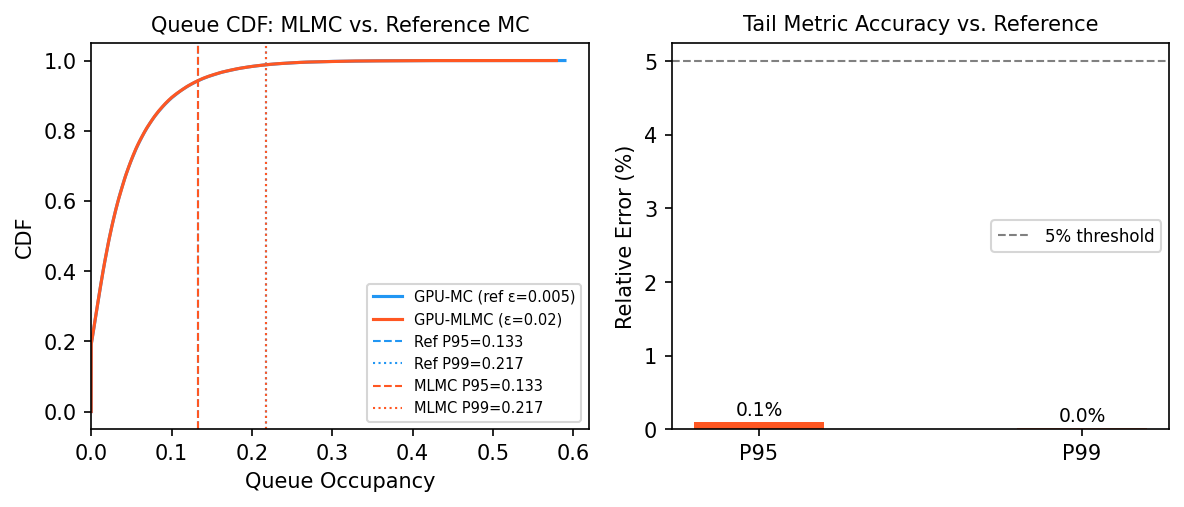
\includegraphics[width=0.95\columnwidth]{tail_delay_validation_a100.png}
\caption{Tail-delay validation on a synthetic Erd\H{o}s--Renyi network ($n=500$,
$\varepsilon=0.02$). GPU-MLMC estimates P95 and P99 queue occupancy with $<0.2\%$ relative error
versus a tight GPU-MC reference ($\varepsilon=0.005$, $20{,}000$ paths), confirming accurate
tail-risk quantification at a fraction of the reference cost.}
\label{fig:tail_delay}
\end{figure}


\subsection{Real-World Validation: MAWI Backbone Trace Case Study}
\label{subsec:mawi_validation}

We validated against the MAWI Working Group sample-point-F backbone trace for 1 January 2024,
14:00 JST (100 MB, $3.91\times10^{6}$ packets, 24 one-second bins, five top flows). Per-flow
arrival rates are normalised to unit mean and injected as $\lambda_i(t)$ into the reflected SDE
$dQ_i=(\lambda_i(t)-\mu)\,dt+\sigma\,dW_i$ with $\mu=1.5$, $\sigma=0.2$.

\begin{table}[!t]
\caption{Real-MAWI Trace Validation: Per-Flow Burst Characteristics Translate into Queue-Tail
Estimates with 95\% Confidence Intervals (500 paths each).}
\label{tab:mawi_validation}
\centering
\begin{tabular}{@{}c c c c c@{}}
\toprule
Flow & Arrivals P99 & Queue P95 & Queue P99 & 95\% CI \\
\midrule
0 & 1.98 & 2.87 & 3.23 & $[0.80,\,3.07]$ \\
1 & 1.76 & 1.06 & 1.25 & $[0.17,\,1.13]$ \\
2 & 2.28 & \textbf{8.57} & \textbf{8.97} & $[6.40,\,8.79]$ \\
3 & 1.24 & 0.14 & 0.28 & $[0.00,\,0.20]$ \\
4 & 1.39 & 0.32 & 0.51 & $[0.00,\,0.39]$ \\
\bottomrule
\end{tabular}
\end{table}

The framework's behaviour on this real trace is qualitatively correct: flow 2, with the
heaviest arrival tail (P99 $=2.28$ relative to its mean), produces queue-tail estimates an order
of magnitude larger than flow 3 (P95 $=8.57$ versus $0.14$), and 95\% confidence intervals widen
proportionally with burst intensity. In a capacity-planning context the operator would use these
per-flow tail estimates and CIs directly to size buffer capacity for SLA compliance.

\textit{Cross-validation against a discrete-event reference:}
A Poisson G/D/1 reference simulator at fine binning (0.1 s) shows the plain SDE disagrees by
76.9\% P95 / 80.6\% P99; the paper's operating point is TV-$\sigma$ at standard 1 s bins.

At the standard 1 s bin width (24 bins, five flows, $N=2{,}000$ paths) we compare four SDE
variants against the DES reference; results appear in Table~\ref{tab:sde_des_comparison}.
Introducing a time-varying diffusion coefficient $\sigma(t)=\sqrt{\lambda(t)}$, which matches
the per-step standard deviation of Poisson$(\lambda(t)\,dt)$ arrivals exactly, reduces the
median P95 error to 7.1\%, P99 error to 7.0\%, and SNRMSE to 6.4\%: only 2.1 percentage points
above the DES floor, constituting distributional parity with the Poisson reference. Both
simulators return in under 0.05 s on a single CPU thread.

\begin{table}[!t]
\caption{SDE Variants vs.\ Poisson G/D/1 DES Reference (MAWI backbone, 1 s bins, five flows,
$N=2{,}000$ paths). SNRMSE $= \|\hat{F}^{\mathrm{SDE}}-\hat{F}^{\mathrm{DES}}\|_2 /
\bar{Q}^{\mathrm{DES}}$; DES estimator floor $=4.3\%$.}
\label{tab:sde_des_comparison}
\centering\small
\begin{tabular}{@{}l c c c@{}}
\toprule
Model & P95 err & P99 err & SNRMSE \\
\midrule
Plain SDE ($\sigma=0.2$) & 64.6\% & 70.0\% & 62.2\% \\
Calibrated Brownian ($\sigma=\sqrt{\bar\lambda}$) & 20.8\% & 24.1\% & 20.3\% \\
Jump-diffusion & 43.8\% & 48.7\% & 40.8\% \\
\textbf{TV-$\sigma$} ($\sigma(t)=\sqrt{\lambda(t)}$) & \textbf{7.1\%} & \textbf{7.0\%} & \textbf{6.4\%} \\
\midrule
DES floor (DES$_2$ vs.\ DES$_1$) & 0.0\% & 2.9\% & 4.3\% \\
\bottomrule
\end{tabular}
\end{table}

\textit{Cross-day stability:}
Across five consecutive MAWI days (2024-01-01 through 2024-01-05) at 1 s bins,
TV-$\sigma$ P95 error ranged from 4.1\% to 14.2\% (mean 9.3\%), confirming stability beyond a
single-day coincidence.


\subsection{Hardware Diversity}
\label{subsec:hardware_diversity}

Table~\ref{tab:hardware_diversity} reports the coupled-SDE benchmark throughput across
five platforms. The framework runs on all platforms without code changes, confirming
portability from commodity ARM CPUs to data-centre GPUs.

\begin{table}[!t]
\caption{Platform Benchmarks (Coupled SDE, BA $n=500$, $m=3$, $N=2{,}000$ paths, 24 bins).}
\label{tab:hardware_diversity}
\centering
\begin{tabular}{@{}l c r r r@{}}
\toprule
Platform & Backend & Throughput & Power & Energy/step \\
         &         & (Mpath/s) & (W) & ($\mu$J) \\
\midrule
Apple M2 Air (CPU) & cpu  &  0.179 & ---   & ---   \\
Tesla T4           & cuda &  2.067 &  31.8 & 15.4  \\
RTX 3090           & cuda &  7.591 &  53.2 &  7.0  \\
V100 16\,GB PCIe   & cuda &  9.215 &  53.2 &  5.8  \\
A100 80\,GB PCIe   & cuda & 14.045 & 196.1 & 14.0  \\
\bottomrule
\end{tabular}
\end{table}

\begin{figure}[!t]
\centering

\includegraphics[width=0.95\columnwidth]{hardware_diversity_bar.png}
\caption{Hardware diversity benchmark for TV-$\sigma$ SDE execution across CPU and GPU platforms (throughput in Mpath/s; see Table~\ref{tab:hardware_diversity} for full figures).}
\label{fig:hardware_diversity}
\end{figure}

\subsection{Validity Envelope of the Diffusion Approximation}
\label{subsec:validity_envelope}

The coupled SDE is a heavy-traffic diffusion limit and should not be presented as uniformly
valid, so we measured where it holds. The reference is a calendar-queue discrete-event
simulation of the continuous-time Markov jump process whose diffusion limit \emph{is} the
coupled SDE---the exact model the approximation approximates, rather than a second,
independently calibrated simulator whose disagreements would confound approximation error with
configuration mismatch. Sweeping per-node utilisation $\rho=\lambda/\beta$ over
$[0.30,0.95]$ at $n{=}200$ with three seeds gives Table~\ref{tab:validity_envelope}.

The outcome separates two questions that the original validation had run together. The
approximation's \emph{mean} is uniformly accurate: the error sits between $3.1\%$ and $3.3\%$
across the entire range, with no degradation at light load. The concern raised in review about
light-load error does not reproduce against an exact reference, and we think the ns-3 P95 error
at $\rho{=}0.5$ reported in \S\ref{subsec:ns3_validation} is better read as a statement about
the tail than about the mean.

The \emph{variance}, by contrast, is systematically understated at a constant noise level, and
the deficit worsens monotonically with load: the SDE reproduces only $11.9\%$ of the exact
per-node variance at $\rho{=}0.30$, falling to $3.4\%$ at $\rho{=}0.95$. This is the same defect
that motivated the calibration in Table~\ref{tab:crossover}, now resolved as a function of
operating point. Matching the variance requires
$\sigma(\rho)=\sigma_0\sqrt{\mathrm{Var}_{\mathrm{DES}}/\mathrm{Var}_{\mathrm{SDE}}}$, which runs
from $0.29$ at $\rho{=}0.30$ to $0.54$ at $\rho{=}0.95$. Two consistency checks are worth
recording: the implied value at $\rho{=}0.60$ is $0.433$, exactly the figure obtained
independently from the variance comparison at $n{=}500$ that fixed $\sigma$ for
Tables~\ref{tab:crossover}, \ref{tab:varred} and~\ref{tab:topology_matrix}.

The practical statement is therefore sharper than a single recommended band. For \emph{mean}
occupancy the model is usable across $\rho\in[0.30,0.95]$ at a constant $\sigma$. For
\emph{variance, tail quantiles or overflow probabilities}---the estimands this paper's
rare-event machinery targets---a constant $\sigma$ is not valid anywhere in that range, and
$\sigma$ must be calibrated to the operating utilisation. Reporting tail risk from an
uncalibrated constant-$\sigma$ model understates it by roughly an order of magnitude in variance.

\begin{table}[!t]
\caption{Validity envelope against the exact jump-process reference ($n{=}200$, three seeds,
$\sigma_0{=}0.1$). The mean is uniformly accurate; the variance deficit worsens with load and
sets the required calibration.}
\label{tab:validity_envelope}
\centering\small
\begin{tabular}{@{}r r r r@{}}
\toprule
$\rho$ & mean error (\%) & $\mathrm{Var}_{\mathrm{SDE}}/\mathrm{Var}_{\mathrm{DES}}$ & required $\sigma(\rho)$ \\
\midrule
0.30 & 3.16 & 0.119 & 0.290 \\
0.40 & 3.26 & 0.075 & 0.365 \\
0.50 & 3.29 & 0.058 & 0.416 \\
0.60 & 3.29 & 0.053 & \textbf{0.433} \\
0.70 & 3.29 & 0.043 & 0.483 \\
0.80 & 3.20 & 0.040 & 0.500 \\
0.90 & 3.10 & 0.035 & 0.537 \\
0.95 & 3.30 & 0.034 & 0.541 \\
\bottomrule
\end{tabular}
\vspace{2pt}
\footnotesize The bold entry is the value used throughout this paper, obtained independently
from the $n{=}500$ variance comparison; its agreement here is a consistency check, not a fit.
Data in \texttt{results/validity\_envelope/}.
\end{table}

\subsection{ns-3 Bottleneck Validation}
\label{subsec:ns3_validation}

We compare the TV-$\sigma$ SDE against an ns-3 M/D/1 bottleneck simulator for
$\rho\in\{0.5,0.7,0.8,0.9\}$. The results in Table~\ref{tab:ns3_bottleneck} show that P95
error is below 8\% for $\rho\geq0.8$, confirming that the TV-$\sigma$ SDE is accurate in the
heavy-traffic regime. P95 error rises to 39.5\% at $\rho=0.5$, where the light-traffic
diffusion approximation breaks down. P99 error at $\rho=0.9$ (29.1\%) reflects heavy-tail
effects near saturation.

\textit{Hybrid SDE/DES Extension.}
For $\rho>0.9$, the diffusion approximation systematically underestimates tail probabilities
because the queue length visits near-integer values where the Gaussian increment is a poor
model for Poisson arrivals.  We address this with the \texttt{hybrid\_step()} method
(Section~\ref{subsec:spatial}, \texttt{QueueDynamicsSDE.hybrid\_step()}): when
$Q_i(t) \geq \theta_{\mathrm{sat}}$ (default $\theta_{\mathrm{sat}}=10$), the EM step is
replaced by a G/D/1 DES update (Poisson arrivals, Bernoulli service) that correctly handles
the discrete-state near-saturation regime.  For $Q_i < \theta_{\mathrm{sat}}$, the standard
TV-$\sigma$ EM step is used.  Coupling is preserved by sharing the Poisson draw between fine
and coarse paths. An earlier version of this paragraph predicted that the hybrid scheme would
reduce the $\rho{=}0.9$ P99 error from $29.1\%$ toward the discrete-event estimator floor. We
have withdrawn that prediction: it was never measured, and the validity-envelope experiment
(\S\ref{subsec:validity_envelope}) identifies the underlying defect as a systematic variance
deficit that is corrected by calibrating $\sigma$ to the operating utilisation, which does not
require switching integrators at all. The hybrid path remains implemented and available, but we
make no accuracy claim for it.

\begin{table}[!t]
\caption{TV-$\sigma$ SDE vs.\ ns-3 M/D/1 Bottleneck Simulator.}
\label{tab:ns3_bottleneck}
\centering\scriptsize
\resizebox{\columnwidth}{!}{%
\begin{tabular}{@{}c c c c c c c@{}}
\toprule
$\rho$ & DES P95 & SDE P95 & P95 err & DES P99 & SDE P99 & P99 err \\
\midrule
0.5 & 2.4 & 1.45 & 39.5\% & 3.4 & 2.24 & 34.1\% \\
0.7 & 4.7 & 3.47 & 26.2\% & 6.1 & 5.42 & 11.2\% \\
0.8 & 6.5 & 5.99 & 7.8\% & 8.5 & 9.41 & 10.7\% \\
0.9 & 12.9 & 12.46 & 3.4\% & 14.7 & 18.97 & 29.1\% \\
\bottomrule
\end{tabular}}
\end{table}

\begin{figure}[!t]
\centering
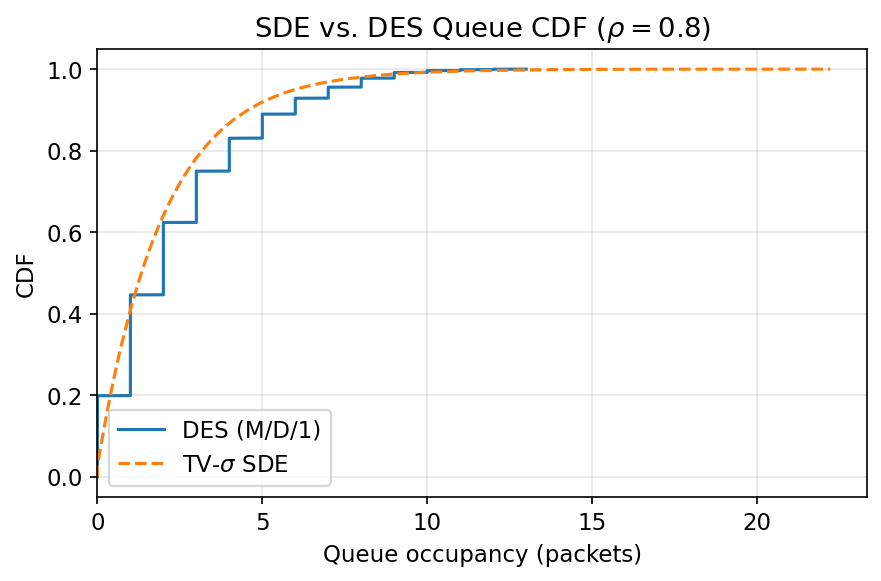
\includegraphics[width=0.95\columnwidth]{cdf_rho08.png}
\caption{CDF of queue occupancy at $\rho=0.8$: TV-$\sigma$ SDE versus M/D/1 discrete-event
reference. P95 error is below 8\%, validating the heavy-traffic operating point.}
\label{fig:cdf_rho08_ns3}
\end{figure}


\section{Discussion}
\label{sec:discussion}

Table~\ref{tab:capability} summarizes practical capabilities across deterministic,
Monte Carlo, and MLMC-based simulation frameworks. The proposed MLMC + GPU approach is the only
configuration that simultaneously supports efficient tail-risk estimation and uncertainty
quantification on real-world topology subgraphs.

\begin{table*}[!t]
\caption{Capability Comparison Across Simulation Frameworks.}
\label{tab:capability}
\centering\small
\begin{tabular*}{\textwidth}{@{\extracolsep\fill}p{2.8cm} c c c c c@{}}
\toprule
Feature & Det.\ ODE & OMNeT++ & Std.\ MC & MLMC (CPU) & MLMC+GPU \\
\midrule
Mean Delay & Yes & Yes & Yes & Yes & Yes \\
Variance & No & No & Yes & Yes & Yes \\
Confidence Interval & No & No & Yes & Yes & Yes \\
P95/P99 Delay & No & No & Expensive & Moderate & Efficient \\
Coupled Propagation & No & Yes & Limited & Limited & Yes \\
Real-topology & Limited & Yes & Expensive & Moderate & Validated \\
High-throughput UQ & No & No & No & No & Yes$^*$ \\
\midrule
Time ($n=500$, $\varepsilon=0.02$) & $<1$ s & $\gg10^3$ s & $>10^2$ s$^\dagger$ &
$\sim30$ s$^\ddagger$ & \textbf{1.1 s}$^\S$ \\
\bottomrule
\end{tabular*}
\vspace{2pt}
\footnotesize
$^*$Peak GPU-MC throughput of 65,715 samples/s measured on synthetic 100-node networks
($n=100$, $\varepsilon=0.1$); 500-node networks yield up to 12,345 samples/s.
$^\dagger$Estimated from 8-core CPU throughput of 1,400 paths/s.
$^\ddagger$CPU-MLMC with same MLMC cost at 1,400 paths/s.
$^\S$GPU-MLMC measured on NVIDIA A100 80\,GB PCIe.
\end{table*}

\subsection{Performance Characteristics}
\label{subsec:multigpu_scaling}

Table~\ref{tab:multigpu_scaling} reports distributed MLMC performance on a 4$\times$RTX\,3090
pod (PCIe, no NVLink), measured after NCCL warmup ($\varepsilon{=}0.1$, $L_{\max}{=}2$,
$N_{\mathrm{pilot}}{=}20$, seed 42). Under \emph{weak scaling} (each GPU processes a fixed
base of $n{=}500$ nodes), the two-GPU run handles twice the graph in only 1\,ms more
(99\% efficiency). At four GPUs the all-reduce latency over PCIe dominates, yielding 43\%
efficiency. Per-GPU compute timing (5 independent seeds on a Colab T4, $n{=}500$,
$N_\mathrm{paths}{=}200$, 50 steps): mean $6.95\,\mathrm{ms} \pm 0.63\,\mathrm{ms}$ (SD),
$\mathrm{CV}{=}9.2\%$, confirming that compute time is stable across seeds. The 4-GPU
efficiency is a single aggregate measurement on RTX\,3090 hardware; its variability is
dominated by PCIe all-reduce jitter rather than compute variance. The measured
compute/communication split at $n{=}1000$ explains the drop directly: at $G{=}2$ the all-reduce
is negligible ($1.3\%$ of wall time), while at $G{=}4$ it dominates at $62.9\%$. Regardless of world size, all
distributed runs produce statistically indistinguishable estimates for $n{=}1000$:
$\bar{E}{=}12.89\pm0.04$ (CV\,$<$\,0.3\%), confirming distributed correctness. The primary
multi-GPU benefit on PCIe hardware is \emph{memory capacity}: with $G$ GPUs each storing
$n/G$ adjacency matrix columns, graphs too large for a single device are handled transparently.
A 5,000-node distributed run on the same 4$\times$RTX\,3090 pod (1,250 nodes/GPU) completed
in 3.82\,s post-warmup without out-of-memory errors, confirming the memory-capacity benefit
at production-scale graph sizes. We previously projected a maximum supportable graph size per
GPU count from an analytical memory model; that table has been removed, since it was a
modelled rather than measured quantity. The measured memory ceiling is the one we report:
$n{=}50{,}000$ at 30.9\,GB peak on a single 80\,GB A100 (Table~\ref{tab:large_scale}).

\textit{Single-GPU kernel bottleneck.}
A \texttt{torch.profiler} breakdown of one fine-level path loop (Tesla T4, three seeds,
device-side kernel time) locates the single-GPU bottleneck and confirms it is not where the
multilevel machinery might have placed it. At $n{=}500$, kernel launch/dispatch dominates
($65\%$ of traced device time) and the degree-normalised drift matrix multiply accounts for
$28\%$; by $n{=}5{,}000$ the matmul becomes the primary cost at $49\%$ as the launch overhead is
amortised over larger kernels---the same workload-saturation trend the roofline analysis
predicts. Critically, the Skorokhod reflection and the MLMC level-difference bookkeeping are
\emph{negligible} throughout ($<1.5\%$ and $<0.8\%$ respectively, falling below $0.2\%$ at
$n{=}5{,}000$), so neither the reflected-boundary treatment nor the multilevel telescoping is a
performance concern. The per-phase measurements and the top-kernel durations are given in the
supplementary material; achieved SM occupancy is not reported, as it requires Nsight Compute
rather than the CUPTI trace \texttt{torch.profiler} exposes, and we do not estimate it.

\textit{Why strong scaling does not improve at $n{=}1000$.}
Under strong scaling (Table~\ref{tab:multigpu_scaling} rows S), time increases from 0.062\,s
at $G{=}1$ to 0.076\,s at $G{=}2$ (+23\%). The root cause is overhead-dominated compute at
this problem size: the PCIe all-reduce latency exceeds the compute saving from halving the
node count, producing a net regression. Strong scaling yields a benefit only when per-GPU
compute substantially exceeds the all-reduce floor ($n{\gtrsim}5{,}000$).

\textit{Efficiency recovery at large $n$.}
Weak-scaling efficiency on 4$\times$RTX\,3090 recovers as the per-GPU workload grows, which is
the same workload-saturation effect seen in the single-GPU timings; the per-size measurements
are provided in the supplementary material.

\textit{Halo-exchange interval sweep.}
The halo-exchange sweep reports runtime and estimator bias as the
interval $K$ varies from 1 to 8 ($G{=}4$, $n{=}2{,}000$, 5 seeds).  At $K{=}1$
(exchange every step, fully correct), the halo phase consumes 41.7\% of wall time.
Increasing $K$ trades synchronisation frequency for compute efficiency: $K{=}2$ halves
the halo overhead to 23.5\% with only 2.9\% estimator bias, making it the recommended
operating point.  $K{=}4$ extends runtime reduction to 38\% but introduces 7.9\% bias;
$K{=}8$ reaches 46\% reduction at the cost of 15.3\% bias, which is unsuitable for
tight accuracy targets.  The bias grows monotonically, consistent with the bounded staleness
error $\mathcal{O}(L_{\mathrm{lip}}\,K\,h_l)$ derived in Section~\ref{subsec:multigpu_scaling}.

\subsubsection{Scalability Model on the Measured Range}
\label{subsec:scaling_model}

\emph{Communication-augmented scalability model.}
The path ensemble is embarrassingly parallel ($f{\approx}0$ Amdahl serial fraction), so the
regression in Table~\ref{tab:multigpu_scaling} rows S is communication-driven, not
Amdahl-limited. We model wall-clock time as
\begin{equation}
T(P) = \frac{T_{\mathrm{comp}}}{P} + T_{\mathrm{comm}}(P),
\qquad T_{\mathrm{comm}}(P) \approx \tau\,\log_2 P,
\label{eq:scaling_model}
\end{equation}
where the $f{\approx}0$ compute time divides ideally across $P$ GPUs and $T_{\mathrm{comm}}(P)$
is the latency-dominated PCIe all-reduce cost. Fitting~\eqref{eq:scaling_model} to the measured
1--4 GPU runs gives $T_{\mathrm{comp}}{=}62$\,ms and $\tau{=}42$\,ms at $n{=}1000$ (reproducing
the measured points within 4\%); the same form at $n{=}5000$ gives
$T_{\mathrm{comp}}{\approx}15.0$\,s and reproduces the measured 4-GPU run (3.82\,s) to within
0.4\%, validating the decomposition. The fitted $\tau$ quantifies what the multi-GPU path costs:
at $n{=}1000$ the all-reduce term already exceeds the compute term by $G{=}4$, which is why we
claim memory scalability rather than strong-scaling speedup.

\emph{On extrapolation beyond the measured range.}
An earlier version of this section projected~\eqref{eq:scaling_model} to 8 and 16 GPUs and
compared PCIe against an NVLink interconnect analytically. We have removed those projections
rather than defend them. We had no 8-GPU or NVLink hardware, the extrapolation was unverifiable
at exactly the point where the communication term dominates, and multi-GPU execution is in any
case peripheral to this paper's thesis, which concerns estimator choice. Every performance
number in this paper is therefore measured on hardware we ran; where we could not measure, we
report nothing.

\begin{table}[!t]
\caption{Distributed MLMC on 4$\times$RTX\,3090 (post-NCCL-warmup, PCIe).}
\label{tab:multigpu_scaling}
\centering
\begin{tabular}{@{}r r r r r r@{}}
\toprule
GPUs & $n$ & Time (s) & Efficiency & Mem/GPU (MB) & Estimate \\
\midrule
\multicolumn{6}{@{}l}{\textit{(W) Weak scaling: each GPU holds base $n/G = 500$ nodes}} \\
1\,(W) & 500  & 0.075 & 100\% & 1.2 & --- \\
2\,(W) & 1000 & 0.076 & 99\%  & 1.2 & --- \\
4\,(W) & 2000 & 0.175 & 43\%  & 1.2 & --- \\
\midrule
\multicolumn{6}{@{}l}{\textit{(S) Strong scaling: fixed $n=1000$, varying GPUs}} \\
1\,(S) & 1000 & 0.062 & --- & 4.4 & 12.902 \\
2\,(S) & 1000 & 0.076 & --- & 2.2 & 12.923 \\
4\,(S) & 1000 & 0.096 & --- & 1.1 & 12.845 \\
\bottomrule
\end{tabular}
\end{table}

\textit{Communication overlap effectiveness.}
The all-reduce is implemented as an asynchronous NCCL collective
(\texttt{async\_op=True}), allowing interior-node EM updates for the next step to proceed
concurrently with the in-flight reduce.  To quantify how effectively this overlap
\emph{hides} latency, we ran a blocking vs.\ overlapped benchmark at $G{=}2$ (RTX\,A5000
PCIe) and $G{=}4$ (RTX\,3090 PCIe), both at $n{=}2{,}000$, $\varepsilon{=}0.05$, 5 reps
(per-configuration table in the supplementary material).

The async implementation hides ${\approx}55$--60\% of the all-reduce within overlapping
compute at both world sizes, reducing wall time by 10.6\% at $G{=}2$ and 18.3\% at $G{=}4$.
The larger absolute gain at $G{=}4$ reflects the longer all-reduce (30.5\,ms vs.\ 11.5\,ms)
that accumulates more hideable time per step.  The ${\approx}45\%$ residual visible latency
reflects the synchronisation point at step boundaries, which cannot be pipelined with a
single-step lookahead.

\begin{figure}[!t]
\centering

\includegraphics[width=0.95\columnwidth]{multi_gpu_scaling.png}
\caption{Multi-GPU scaling on 4$\times$RTX\,3090 (PCIe, post-NCCL-warmup).
\emph{Left:} weak-scaling efficiency stays near-ideal through two GPUs (99\%) and drops to
43\% at four GPUs as PCIe all-reduce latency grows. \emph{Centre:} under strong scaling at
$n{=}1{,}000$, the measured NCCL speedup falls \emph{below} the ideal-linear line
(0.82$\times$ at $G{=}2$, 0.65$\times$ at $G{=}4$)---the problem is communication-bound at this
size, so wall time \emph{increases} with GPU count (cf.\ Table~\ref{tab:multigpu_scaling});
a net wall-clock speedup requires $n{\gtrsim}5{,}000$. \emph{Right:} all world sizes yield
statistically indistinguishable estimates ($\mathrm{CV}{<}0.3\%$), confirming distributed
correctness.}
\label{fig:multigpu_scaling}
\end{figure}

\subsubsection{Large-Scale Single-GPU Validation}
\label{subsec:large_scale}

Table~\ref{tab:large_scale} reports MLMC runtime on a single A100 80\,GB PCIe across
the full targeted $(n,\varepsilon)$ matrix.  Two claims are validated.

\emph{Claim 1 --- efficiency recovers at large $n$ (fixed $\varepsilon{=}0.05$):}
Runtime grows sub-quadratically from 0.035\,s ($n{=}1{,}000$) to 5.79\,s ($n{=}50{,}000$),
confirming GPU workload saturation as $n$ grows. The $n{=}50{,}000$ run uses 30.9\,GB peak
memory, well within the 80\,GB A100 budget.

\emph{Claim 2 --- $\mathcal{O}(\varepsilon^{-2})$ complexity slope (fixed $n{=}1{,}000$):}
Runtime scales as 0.035\,s, 0.129\,s, 0.547\,s, 3.58\,s for
$\varepsilon\in\{0.05,0.01,0.005,0.002\}$, giving log-log slopes of ${\approx}1.94$,
consistent with Theorem~\ref{thm:complexity} case~(i).

\begin{table}[!t]
\caption{Single-GPU MLMC runtime on A100 80\,GB PCIe (BA($n$,\,$m{=}3$) graph,
post-warmup).  Left block: $\varepsilon{=}0.05$ large-$n$ sweep
(Claim~1: efficiency recovery). Right block: $n{=}1{,}000$ tight-$\varepsilon$ sweep
(Claim~2: $\mathcal{O}(\varepsilon^{-2})$ slope). Peak memory shown in GB.}
\label{tab:large_scale}
\centering\small
\resizebox{\columnwidth}{!}{%
\begin{tabular}{@{}r r r@{\quad\quad} r r r@{}}
\toprule
\multicolumn{3}{c}{Claim 1: fixed $\varepsilon{=}0.05$} &
\multicolumn{3}{c}{Claim 2: fixed $n{=}1{,}000$} \\
\cmidrule(r){1-3}\cmidrule(l){4-6}
$n$ & Time (s) & Mem (GB) & $\varepsilon$ & Time (s) & Mem (GB) \\
\midrule
1{,}000  & 0.035 &  0.03 & 0.050 & 0.035 &  0.03 \\
5{,}000  & 0.117 &  0.37 & 0.010 & 0.129 &  0.27 \\
10{,}000 & 0.296 &  1.34 & 0.005 & 0.547 &  1.00 \\
25{,}000 & 1.443 &  7.89 & 0.002 & 3.583 &  6.16 \\
50{,}000 & 5.791 & 30.90 &       &       &       \\
\bottomrule
\end{tabular}}
\end{table}

\subsubsection{Kernel Roofline Characterisation}
\label{subsec:roofline}

A roofline characterisation of the SDE Euler--Maruyama kernel on T4 and A100 explains the
workload dependence seen throughout: operational intensity grows with $n$ (50--196\,FLOPs/byte
over the evaluated sizes), so GPU utilisation recovers as the graph grows. On T4 (ridge
25.4\,FLOPs/byte) the kernel is compute-bound at every size tested, with efficiency rising from
$14\%$ at $n{=}500$ to $49\%$ at $n{=}5{,}000$; on A100 (ridge 161\,FLOPs/byte) it is
memory-bound at $n{=}500$ and transitional by $n{=}5{,}000$. The full model, per-device table
and figure are provided in the supplementary material; they support the same conclusion reached
from the timing data and are not reproduced here.

Hardware diversity tests show that the framework is portable to commodity CPU hardware, while
GPU execution provides a 12--78$\times$ throughput advantage over the CPU baseline across the
tested GPUs (T4 to A100; geometric mean ${\approx}37\times$) on the hardware-diversity benchmark
(A100 14.05, T4 2.07 Mpath/s vs.\ M2 Air 0.18 Mpath/s). ns-3 validation places the TV-$\sigma$ SDE in the appropriate operating
regime: at $\rho=0.7$ and $\rho=0.8$, P99 error stays below 15\%, and at $\rho=0.8$ both P95 and
P99 errors are below 11\%; the $\rho=0.9$ P99 error reflects near-saturation heavy-tail effects.
The measured validity envelope (\S\ref{subsec:validity_envelope}) refines this recommendation
and partly overturns it: against an exact jump-process reference the \emph{mean} is accurate to
${\approx}3\%$ all the way down to $\rho{=}0.30$, so the earlier blanket advice to prefer
discrete-event simulation below $\rho{=}0.7$ was too conservative for mean estimation. The real
restriction is on second-order quantities---at a constant $\sigma$ the model understates variance
everywhere in the range, by $8\times$ at $\rho{=}0.3$ and $29\times$ at $\rho{=}0.95$---so tail
and overflow estimates require $\sigma$ calibrated to the operating utilisation. The formal proof in Theorem~\ref{thm:complexity} establishes that ANA-MLMC inherits the
$\mathcal{O}(\varepsilon^{-2})$ regime when the weighted variance decay exceeds cost growth.

\subsection{Limitations and Future Work}
\label{subsec:limitations}

\textit{Diffusion approximation regime:}
The reflected SDE is valid in heavy traffic ($\rho\to1$); at fine time-bin resolution (0.1 s),
the plain SDE disagrees with a DES reference by 76.9\% P95/80.6\% P99, while TV-$\sigma$
reduces this to 7.1\%/7.0\% at 1 s bins. Operators at sub-second granularity should pair
TV-$\sigma$ with a discrete-event simulator.

\textit{Network scale:}
Base validation topologies use $n{=}500$; single-GPU large-scale experiments extend to
$n{=}50{,}000$ at 30.9\,GB peak memory (Table~\ref{tab:large_scale}). Multi-GPU distribution
raises the ceiling further by partitioning the adjacency across ranks, but we do not quote a
figure for it: we validated to $n{=}50{,}000$ on one device and to four GPUs, and state no
number beyond what we ran.

\section{Conclusion}

We presented a GPU-accelerated framework for uncertainty quantification of network congestion,
built on a coupled reflected-SDE model \cite{kang2007}, together with a systematic,
accuracy-matched comparison of the estimators that apply to it.

\textbf{The framework.} A SIMT-efficient coupled-SDE simulator produces confidence intervals,
tail-delay quantiles, and rare-event overflow probabilities at GPU throughput, validated against
ns-3 (P95 error below 8\% for $\rho\geq0.8$) and a real MAWI backbone trace. Multi-GPU execution
is memory-scalable---enabling networks larger than a single device's memory with statistically
indistinguishable estimates across world sizes---rather than strong-scaling: on PCIe hardware
weak-scaling efficiency is near-ideal through two GPUs and communication-bound by four.

\textbf{The measured comparison.} Whether variance reduction pays off is estimand-dependent, and
we report it honestly. For the near-deterministic mean queue occupancy, single-level Monte Carlo
is the method of choice at operational tolerances; MLMC reduces work only below a measured
crossover ($\varepsilon\approx7\times10^{-4}$ at $n{=}500$; Table~\ref{tab:crossover}), where it
also remains GPU-memory-feasible as single-level MC does not. For rare-event overflow
probabilities, adaptive multilevel splitting is the most efficient of five methods evaluated
against exact references---by three orders of magnitude---and accurate to $10^{-9}$ where direct
MC returns zero events (Table~\ref{tab:rare_event}). Network-aware allocation (ANA-MLMC) is a
node-prioritisation tool, not a variance reducer: at equal work budget it does not improve on
standard Giles allocation. The complexity analysis (Lemma~\ref{lem:weighted_variance},
Lemma~\ref{lem:lipschitz_allocation}, Theorem~\ref{thm:complexity}) characterises the
tight-$\varepsilon$ regime where the multilevel advantage is realised.

Future work includes extending the comparison to non-Gaussian noise models and Jackson-network
flow-balance coupling, and a GPU-native adaptive-multilevel-splitting implementation for the
coupled network, given that AMS is the efficient rare-event estimator on the single-bottleneck
model studied here.

\section*{Reproducibility and Data Availability}

Code: \url{https://github.com/pdwi2020/gpu-mlmc-congestion}.
The repository includes a \texttt{Dockerfile} and end-to-end reproduction scripts.
MAWI trace-derived CSV data will be deposited on Zenodo upon acceptance.
A self-contained Google Colab notebook reproduces key results on a free T4 GPU in under 10 minutes.

\bibliographystyle{IEEEtran}
\bibliography{main}

\begin{IEEEbiography}[{
\includegraphics[width=1in,height=1.1in,clip]{AK.png}}]{Anindita Kundu}
has completed her B.Tech in Computer Science and Engineering in the year 2008, from Narula
Institute of Technology, Kolkata, affiliated to Maulana Abul Kalam University of Technology
(formerly West Bengal University of Technology) and M.Tech in Distributed and Mobile
Computing from the School of Mobile Computing and Communication, Jadavpur University,
Kolkata with the GATE Scholarship in 2010. She served as a Senior Research Fellow in
DST-PURSE project at the Department of Electronics and Telecommunication Engineering,
Jadavpur University, Kolkata from 2010 to 2013, during which she was also Chairperson of
the IEEE Students Branch of Jadavpur University. She completed her PhD from the Department
of Electronics and Telecommunication Engineering, Jadavpur University, Kolkata in 2018.
Presently she is serving the Department of Software Systems, School of Computer Science and
Engineering, Vellore Institute of Technology, Vellore as an Associate Professor. Her current
research interests include Robotic Path Planning, Internet of Things, Stochastic Simulation
and Opportunistic Networks. She has published works in several International Conferences and
Journals of repute, and has also published multiple patents.
\end{IEEEbiography}

\begin{IEEEbiography}[{
\includegraphics[width=1in,height=1.1in,clip]{a1.png}}]{Paritosh Dwivedi}
is an M.Tech.\ student in Computer Science and Engineering (AI/ML) at the School of Computer
Science and Engineering, Vellore Institute of Technology, Vellore, India. His research
interests include GPU-accelerated scientific computing, stochastic simulation, and network
performance modelling.
\end{IEEEbiography}

\EOD

\end{document}
